%================================================================
%\documentclass{article}%[article,accept,moreauthors,pdftex,10pt,a4paper]{Definitions/mdpi}
\documentclass[article,accept,moreauthors,pdftex,10pt,a4paper]{../MDPI_template/Definitions/mdpi}
%\usepackage[lite]{mtpro2}
\usepackage{scalerel}
\firstpage{1} 
\makeatletter 
\setcounter{page}{\@firstpage} 

\Title{Energy Equalization using Lost Muons}
\Author{Nandita Raha, Marco Incagli \\$INFN ~Pisa$}
% Authors, for the paper (add full first names)

\abstract{
The Muon g-2 experiment at Fermilab will measure the 
anomalous magnetic moment of the muon to a precision of 140 parts per billion (ppb) 
\cite{TDR} compared to the previous measurement at 540 ppb of E821 
by increasing statistics and using upgraded apparatus. 
The maximum allowed systematic uncertainty in the measurement of the spin precession 
frequency $\omega_a$ is 70 ppb which depends on the accurate measurement of the energy 
spectrum of the decay positrons. This, in turn, depends on the proper energy calibration and 
equalization of the calorimeters used for this measurement. The experiment uses 24 calorimeters 
surrounding the penning trap with 54 $PbF_2$ crystals for each calorimeter, thus comprising of 
1296 crystals. 
The energy equalization pertains to the alignment of the energy deposited 
(either by lost muons or endpoint energy of decay positrons) in all crystals to the 
same value. This can be done using various methods. 
This document checks the validity of the equalization procedure 
established for all crystals for run 1 data using the lost muon energy 
spectrum. Muons lose energy all around the storage ring (or penning trap) due to interaction 
with various components like the collimators at the entrance of the ring etc. 
These muons behave as minimum ionizing particles (MIP) and 
deposit energies of 170 MeV in $PbF_2$ \cite{c3}. We use a dataset to define a set of equalization 
constants and apply them to other datasets of run1 and check if any correction is necessary.}
\begin{document}
%\setcounter{section}%{} %% Remove this when starting to work on the template.

\section{Introduction}
\noindent To ensure the required precision of the experiment, the energy spectrum obtained 
from all the crystals of all the calorimeter must be consistent. This would enable 
adding the energy spectra of all crystals to generate the final energy spectrum. 
In order to achieve this consistency, the energy scales of individual channels are aligned
by using the lost muon peak of the energy distribution. This process is called energy equalization. 
Here we investigate this equalization and check its consistency across various datasets. Further, we 
explore the possibility of defining new energy equalization constants and check if these will improve 
our final result and if it will actually be essential to incorporate them in the future reconstruction.

\section{Lost muons - energy spectrum of triplets}
\noindent The lost muons can move through any number of calorimeters before actually stopping 
in a calorimeter. We consider muons traversing exactly three calorimeters before stopping completely. 
These triple coincidences having a time 6.2 ns \cite{docdb16402} between consecutive calorimeters are tagged as triplets 
and used for this analysis. The details of the lost muon definition can be found in \cite{docdb16402}. 
We additionally required that there should be a single hit in the cluster of the lost muon event for the triplets.  
Muons of 3.1 GeV energy deposit an energy of about 170 MeV in $PbF_2$ crystals. The energies deposited 
in the three consecutive calorimeters by a lost muon event are E0, E1 and E2 respectively, where E0 is 
the energy deposited in the last calorimeter. The left panel of figure \ref{fig1} 
shows a lost muon event where the last hit is in calorimeter 3. 
The middle and right panels of figure \ref{fig1} show two other lost muon events 
where the last hits are in calorimeters 4 and 5 respectively. 
\begin{figure}[H]
\centering
%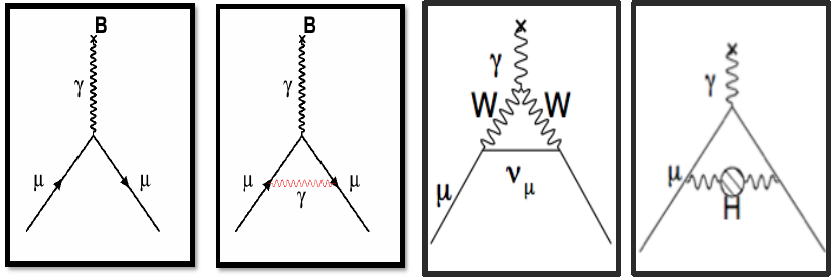
\includegraphics[width=2 cm]{a_mu_corrections.png}
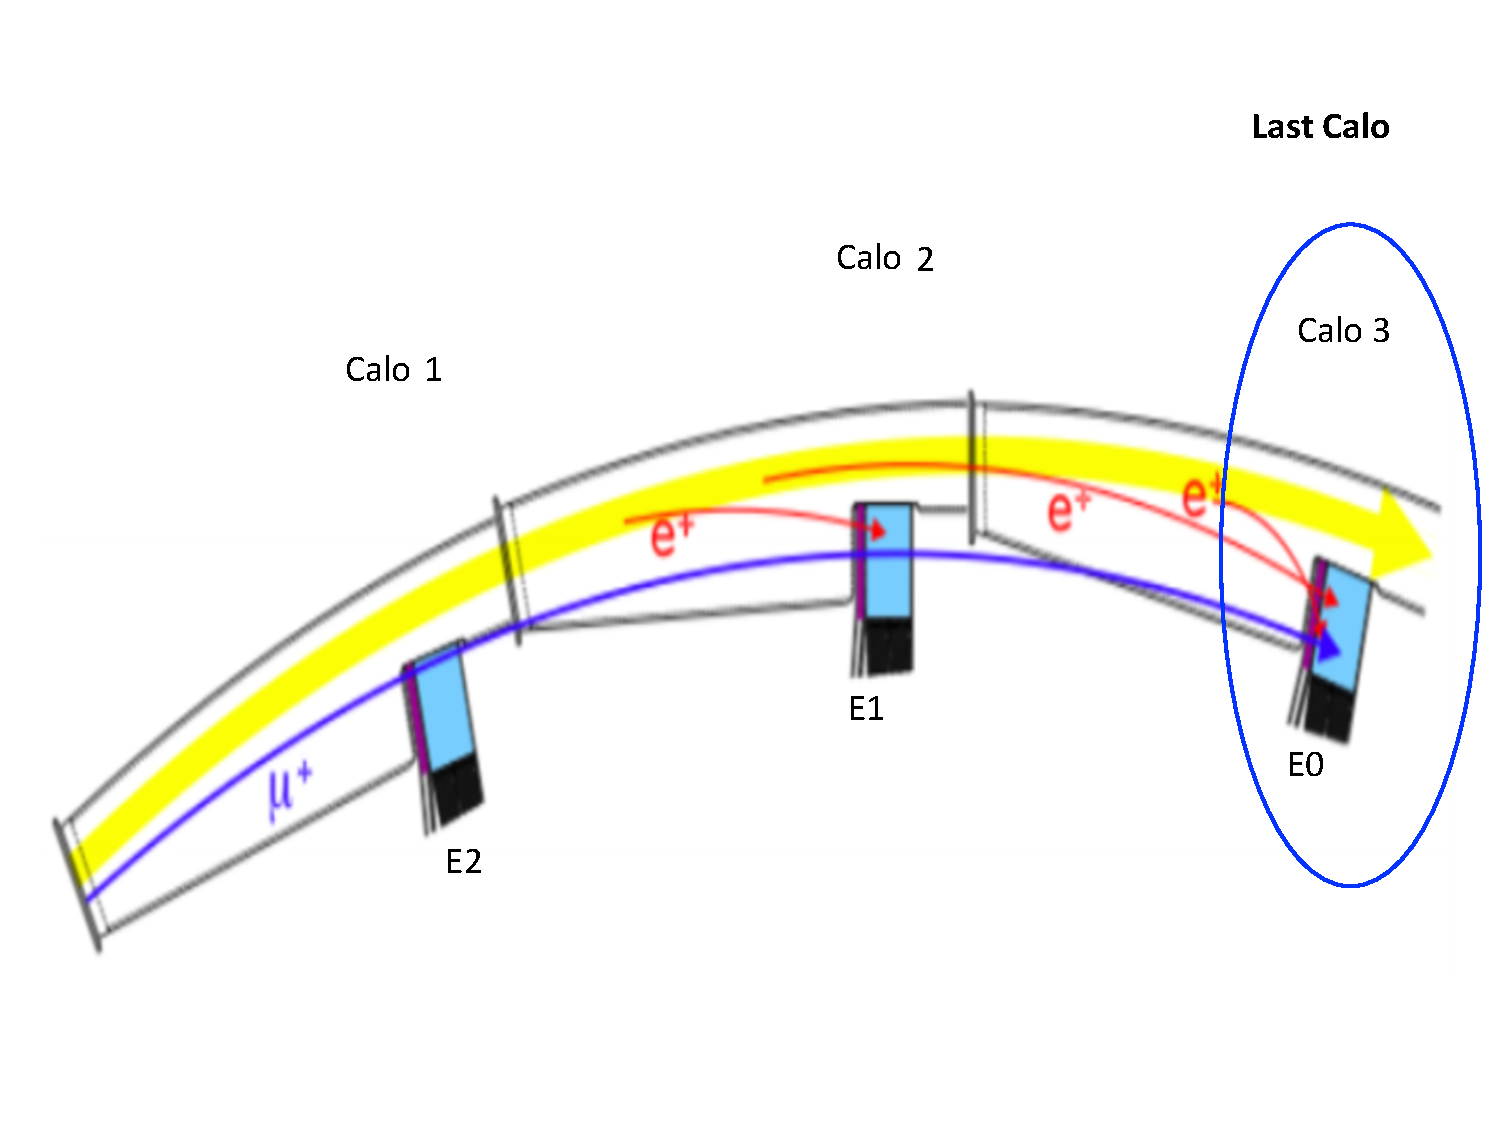
\includegraphics[width=5 cm]{E0.pdf}
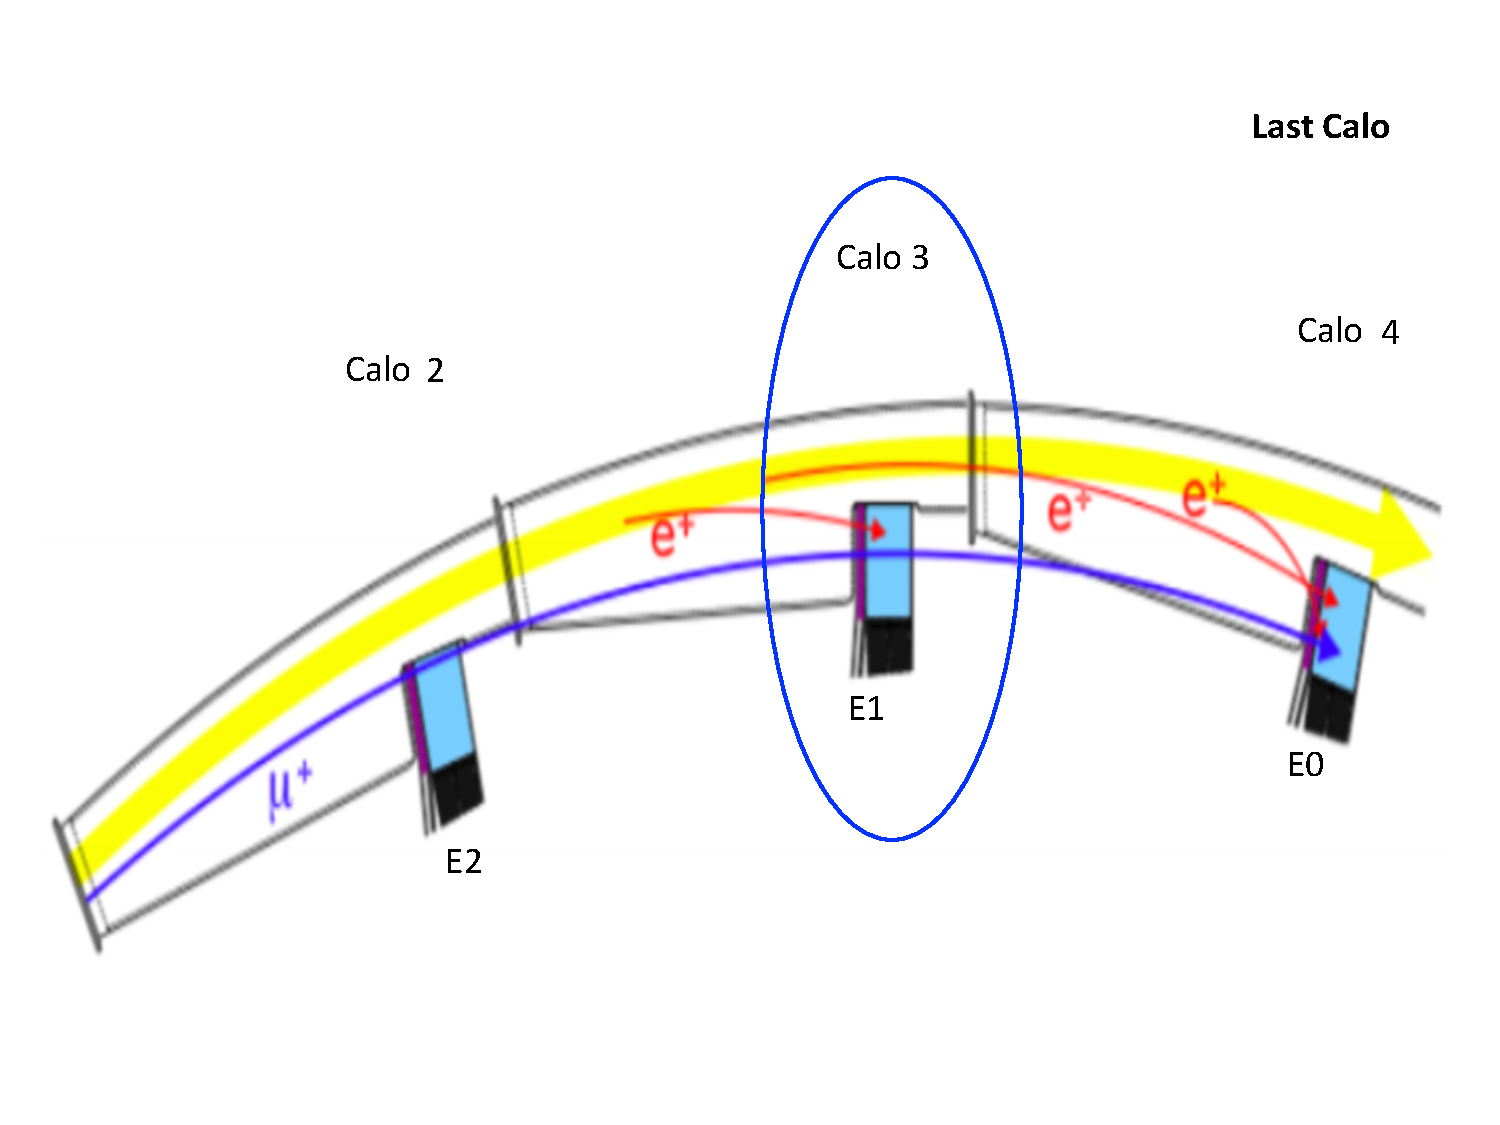
\includegraphics[width=5 cm]{E1.pdf}
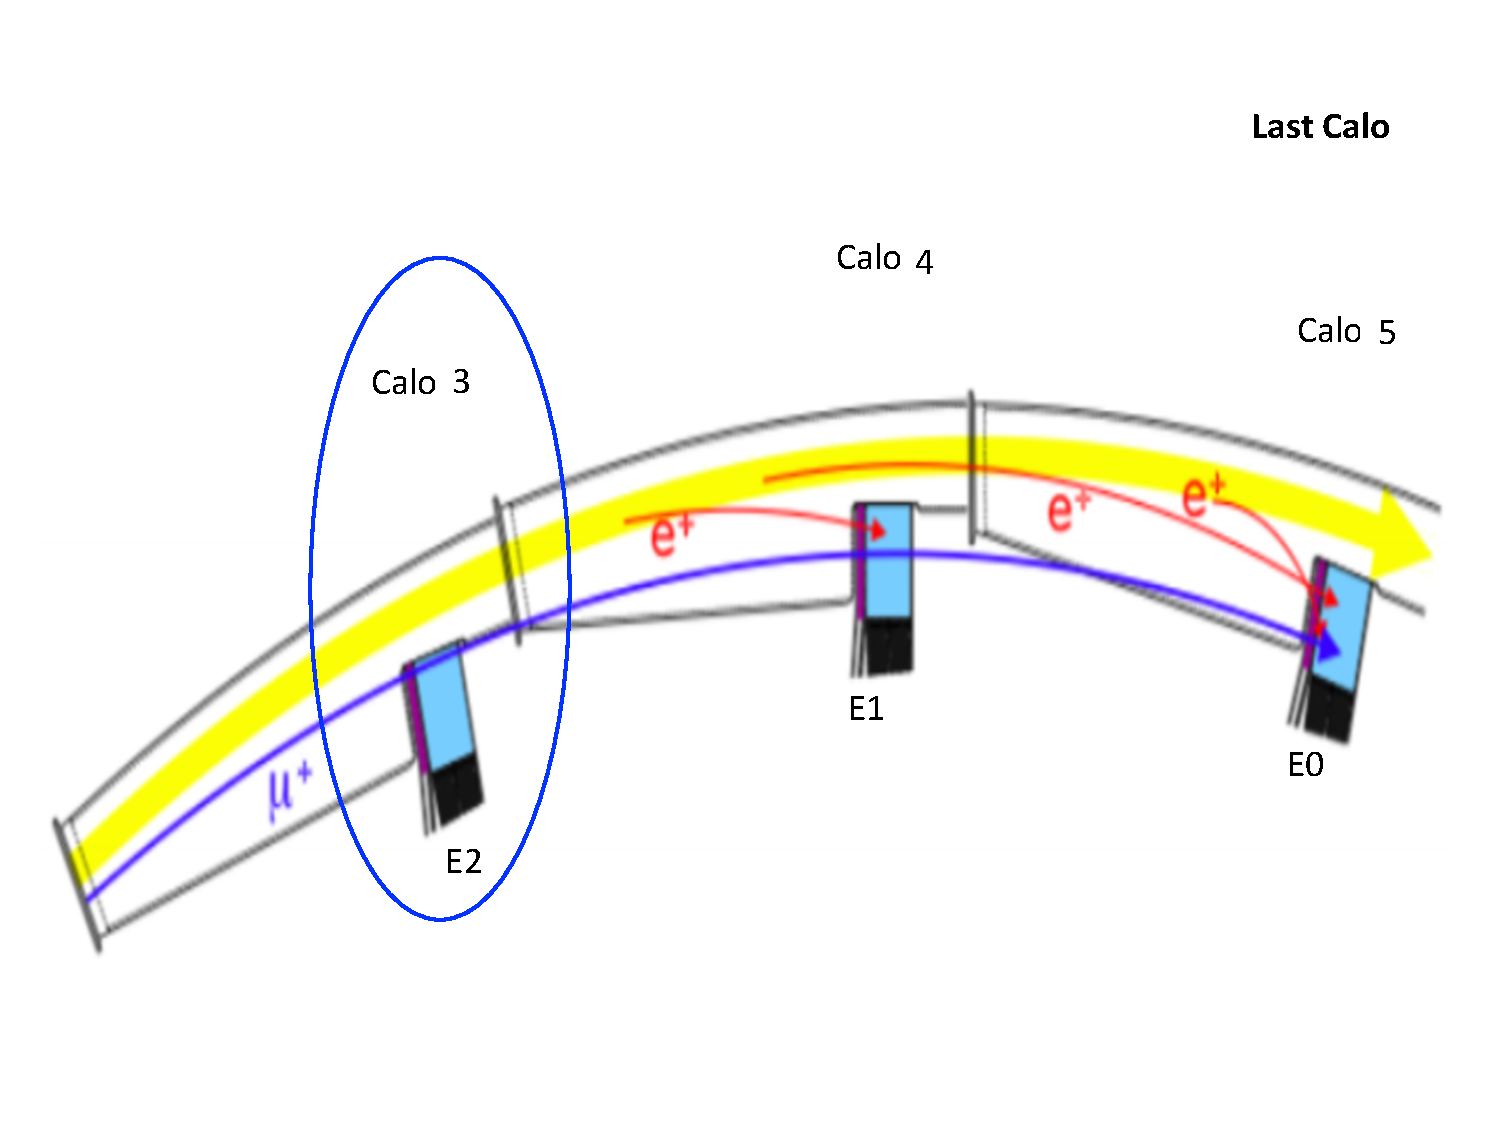
\includegraphics[width=5 cm]{E2.pdf}
%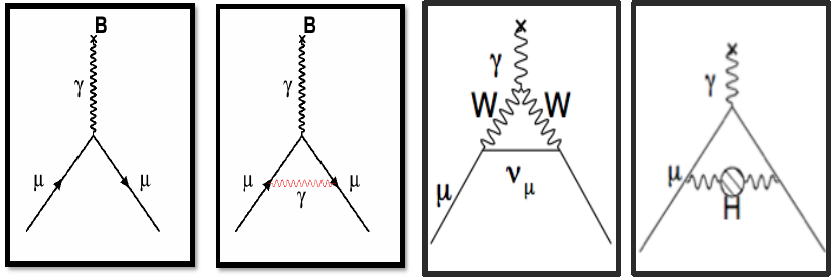
\includegraphics{a_mu_corrections.pdf}
\caption{\label{fig1} All three energies E0, E1 and E2 of the triple coincidence of a muon loss 
event passing through calorimeter 3. }
\end{figure}  

Thus for these three lost muon events E0, E1 and E2 correspond to hits in the same calorimeter 3. 
To increase the statistics of a particular calorimeter we accumulate the energies E0, E1 and E2 deposited 
by three such lost muon events.
Figure \ref{fig3} shows the spectrum of E0, E1 and E2 for these three lost muon events for calorimeter 1 crystal 22 of a 
60--hour dataset. These compare reasonably well (the peaks align well and thus these energy distributions/histograms can be 
accumulated for higher statistics).
%\begin{figure}[H]
%\centering
%\includegraphics[width=11 cm]{Energy_overlaid.pdf}
%\caption{\label{fig2}The energy spectrum of triple coincidences of lost muons for all three energies E0, E1 and E2.}
%\end{figure} 

A small range about the peak is fitted with a Gaussian to get the MIP peak of the triplets. This is a 
reasonable procedure to find the peak as the reduced $\chi^2$ is acceptable. Figure \ref{fig3} shows 
the reduced $\chi^2$ of the spectra due to E0, E1 and E2 are 1.02, 0.72 and 0.9 respectively for this crystal. 
The final combined spectra \ref{fig3}(d) has a relatively higher reduced $\chi^2$ of 0.7. This figure also shows 
no significant difference in the MIP peaks for E0, E1, E2 and their combination. 
This is true for all crystals of every calorimeter and justifies combining the spectra E0, E1 and E2 for the same crytal. 

\begin{figure}[H]
\centering
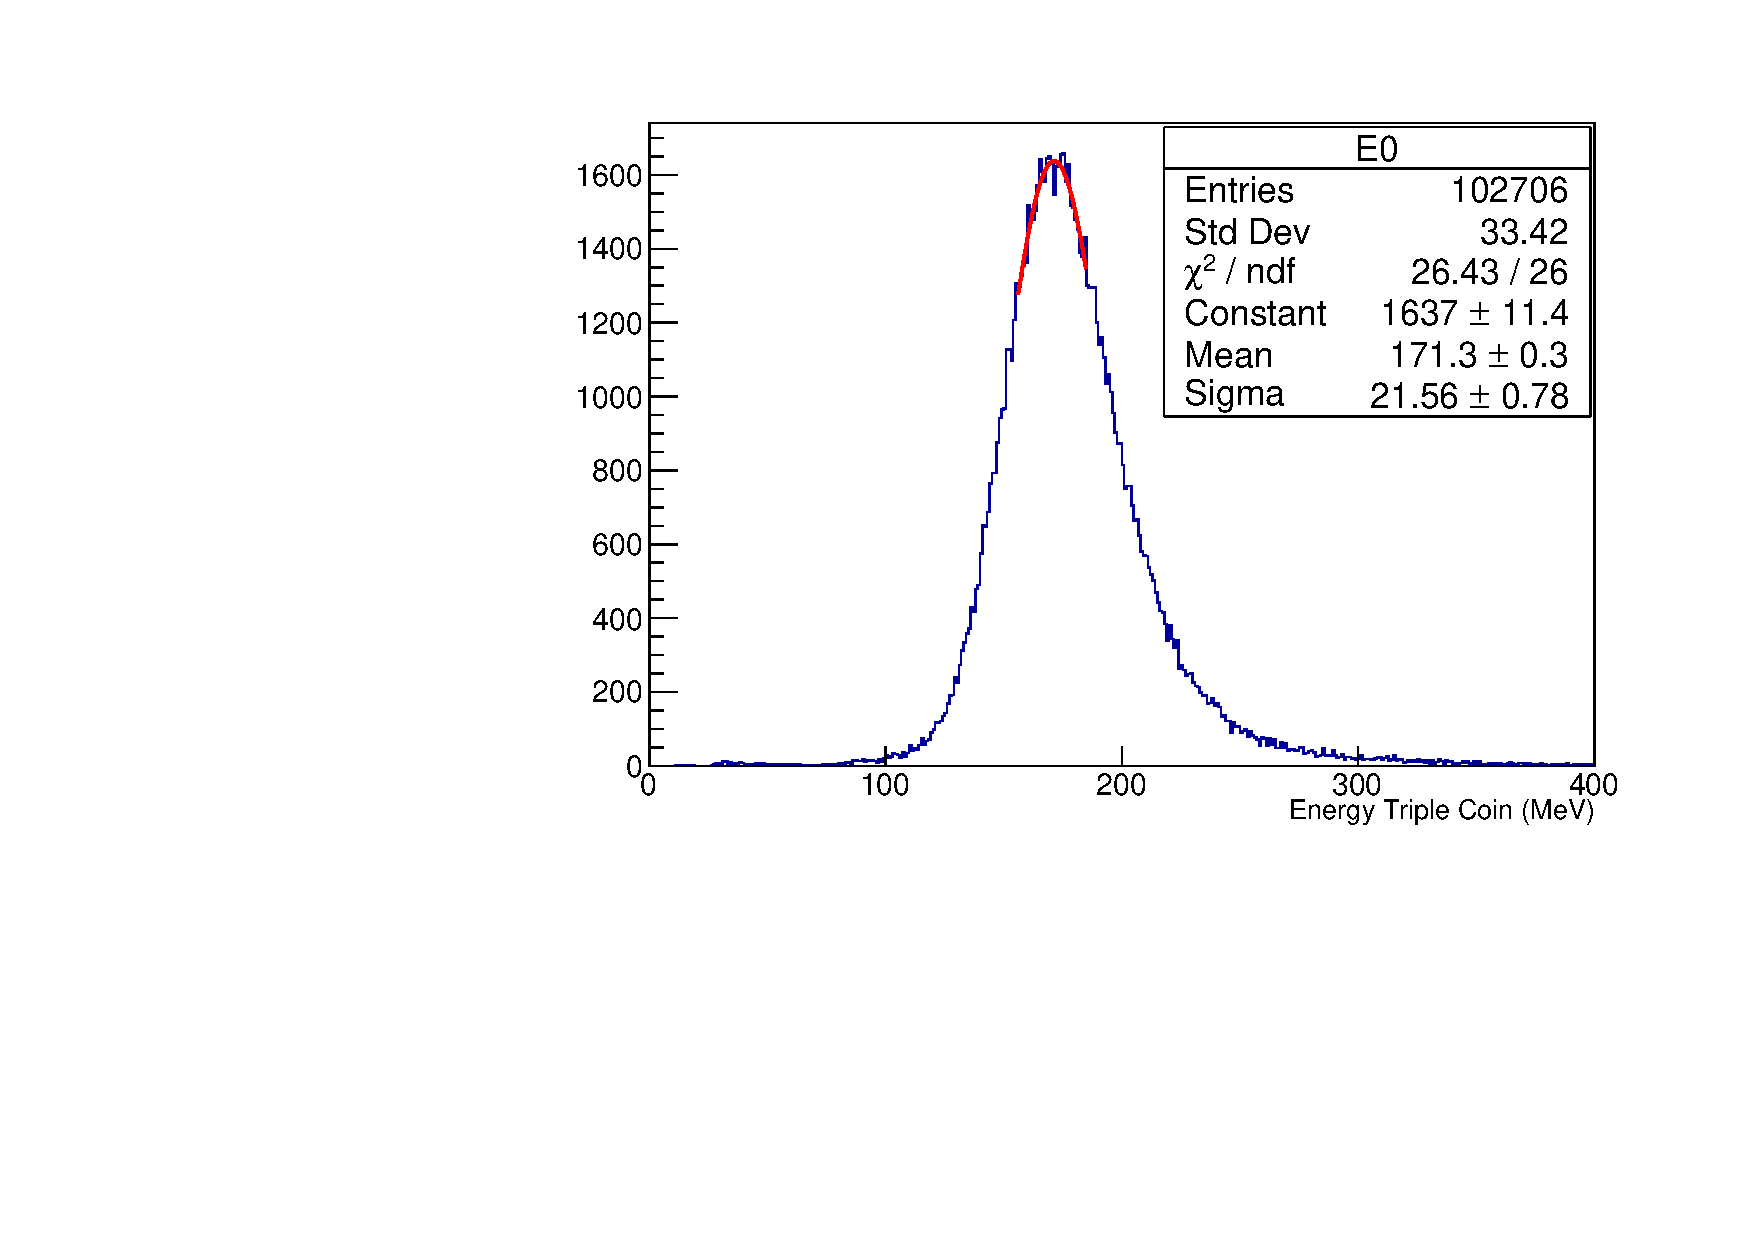
\includegraphics[width=7.5 cm]{calo1_E0.pdf}
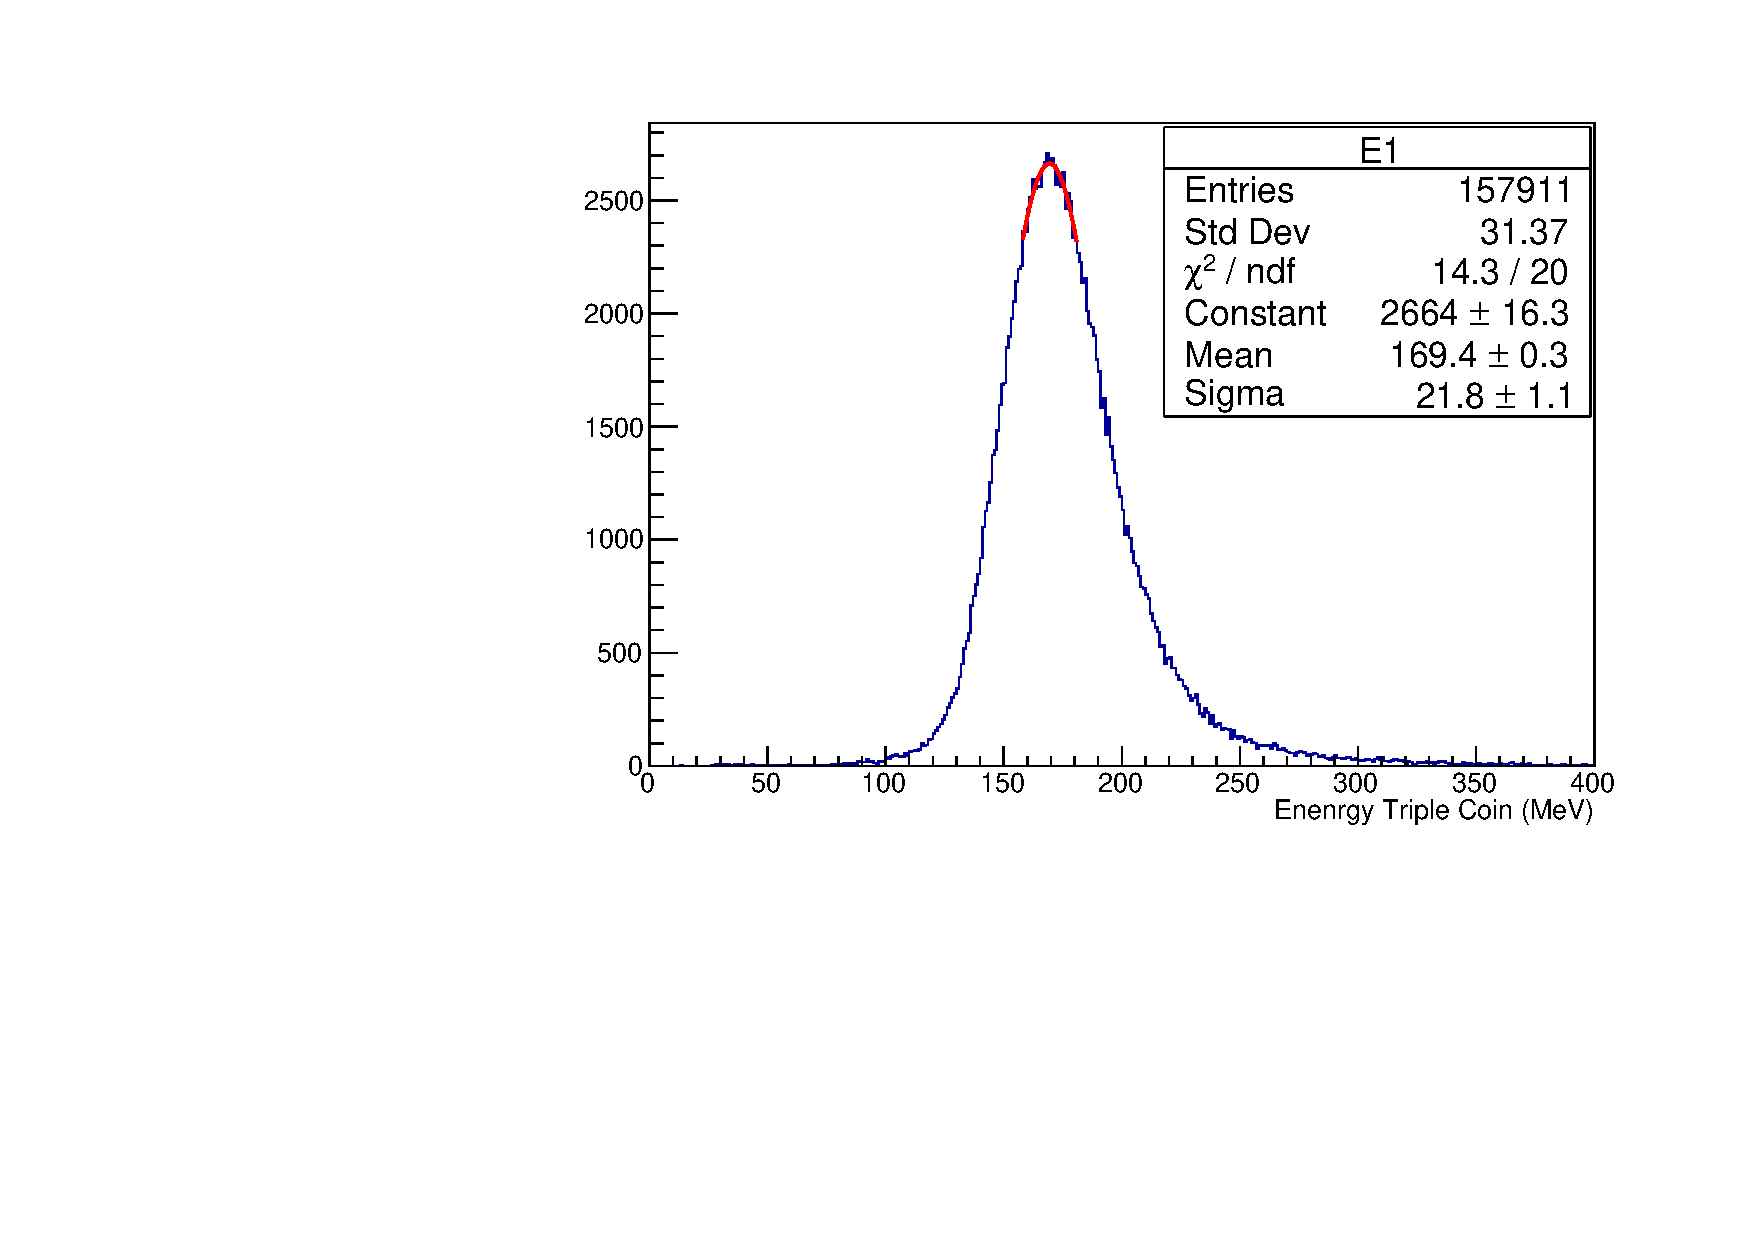
\includegraphics[width=7.5 cm]{calo1_E1.pdf}\\
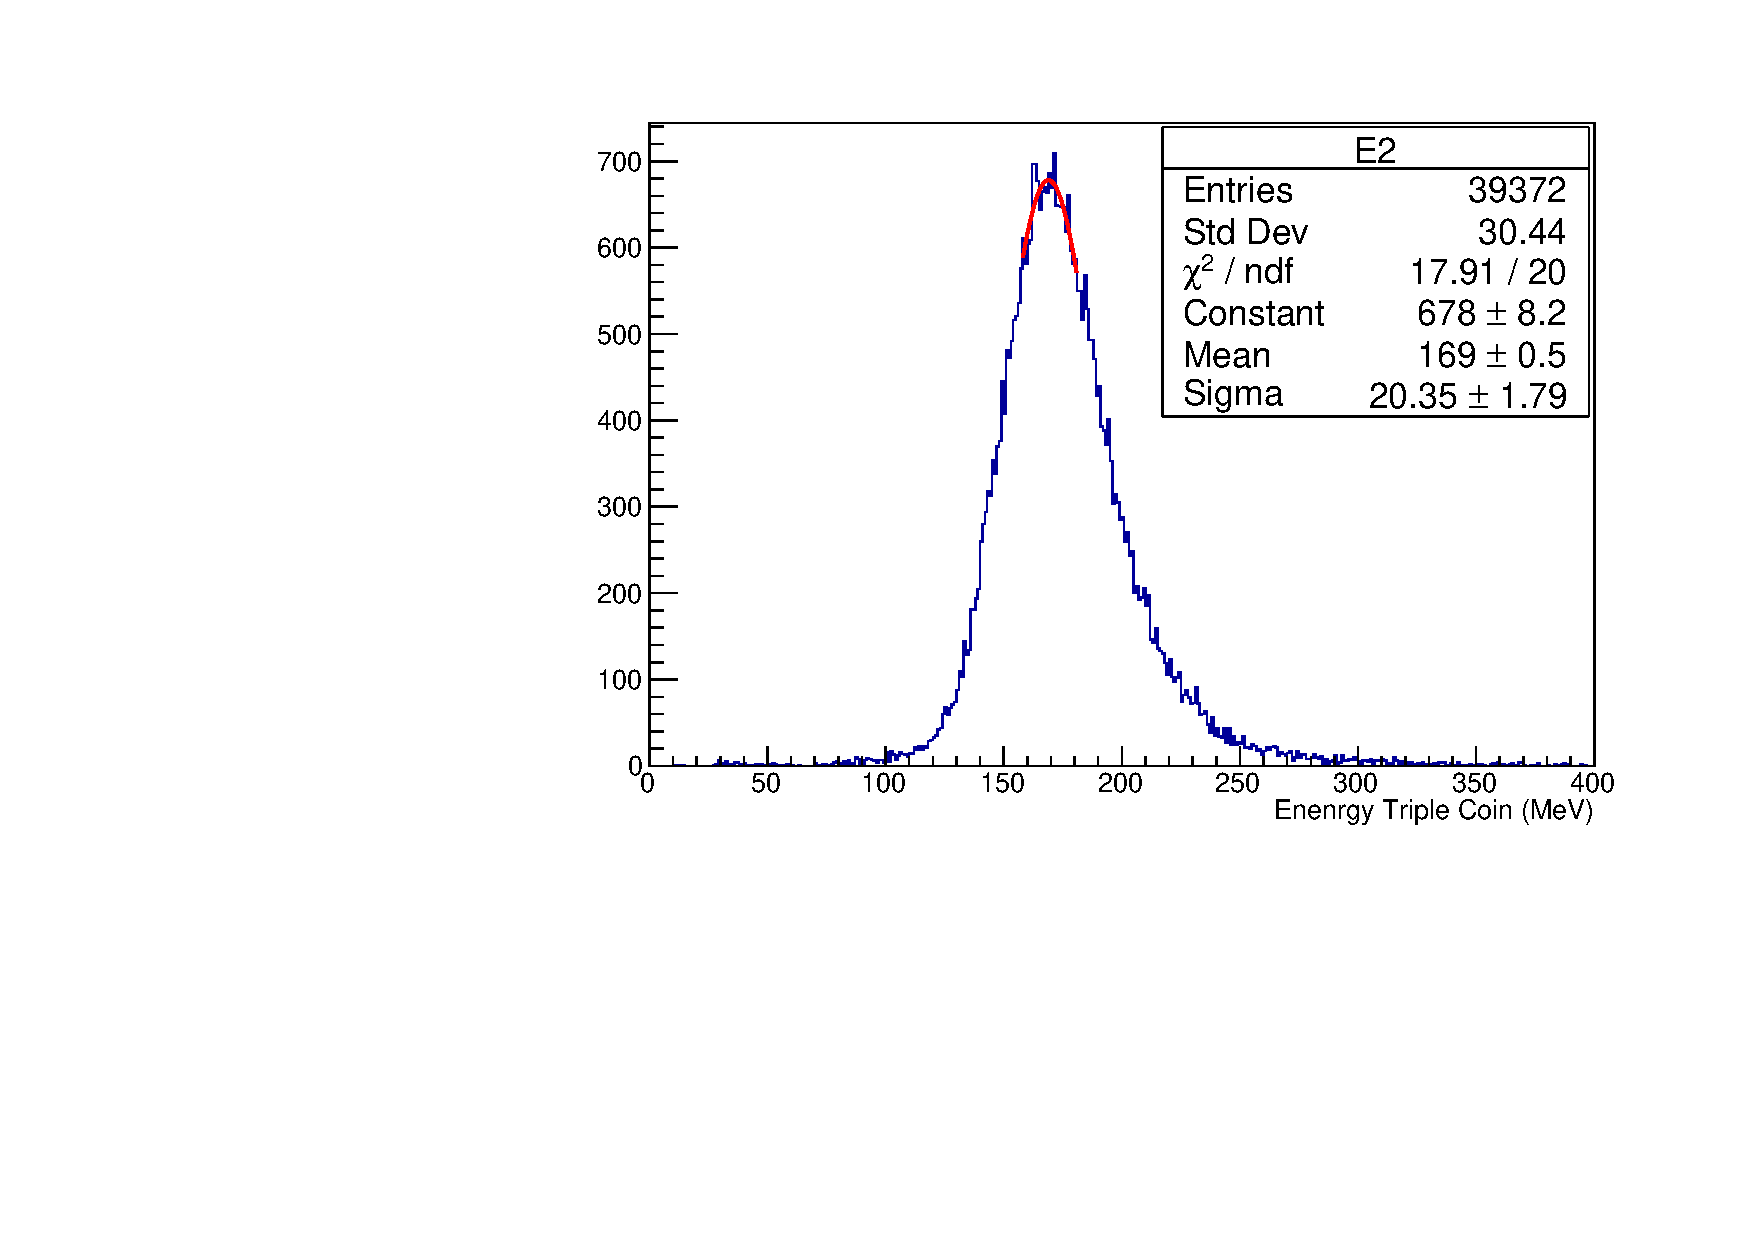
\includegraphics[width=7.5 cm]{calo1_E2.pdf}
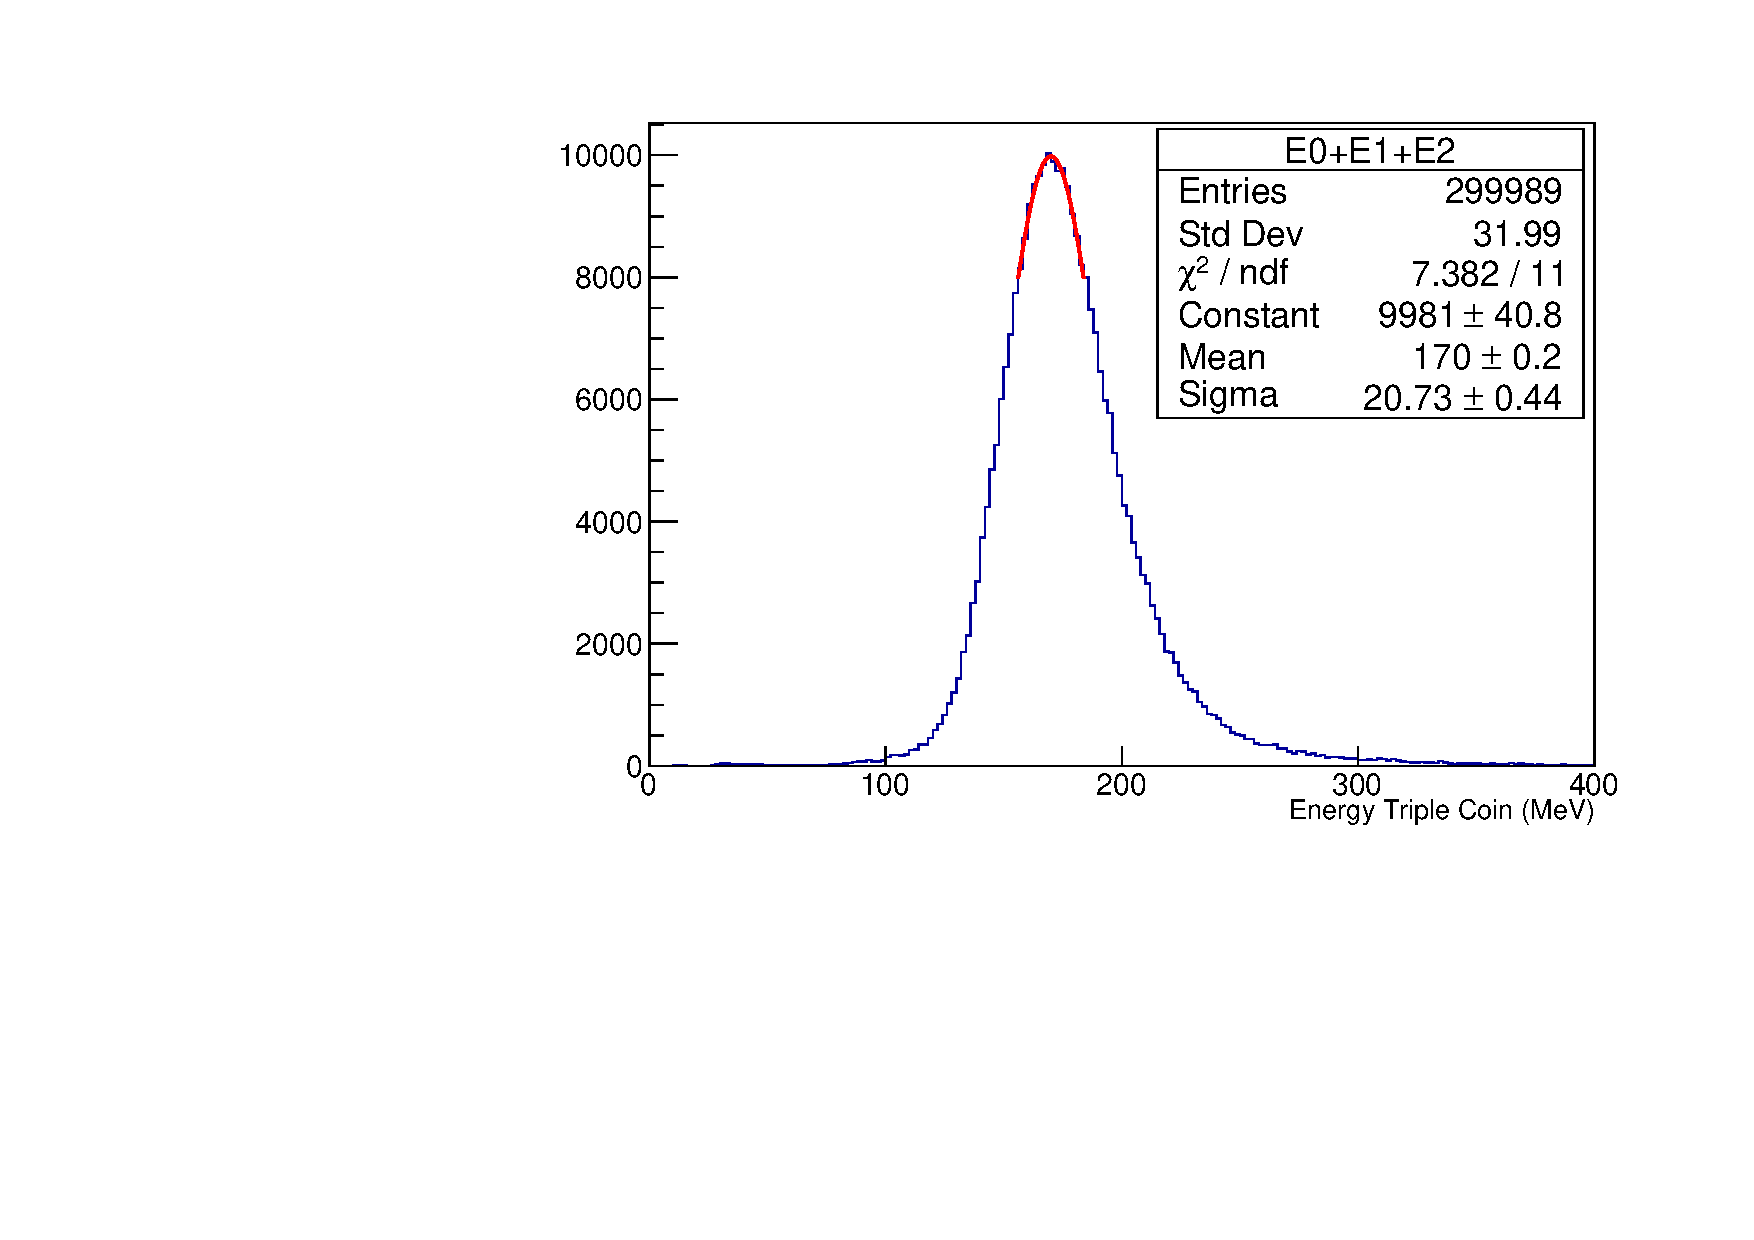
\includegraphics[width=7.5 cm]{calo1_all.pdf}
%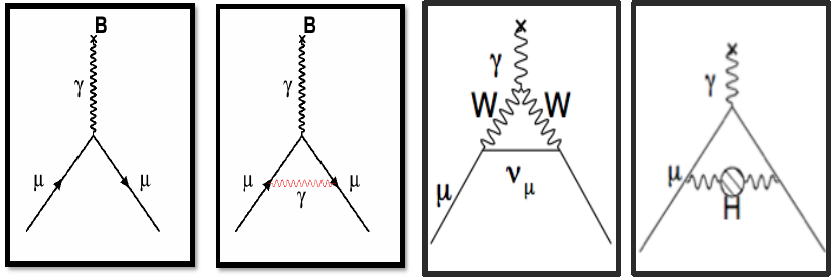
\includegraphics{a_mu_corrections.pdf}
\caption{\label{fig3} A Gaussian fit about the peak for spectra of triplets E0, E1 and E2 for calorimeter 1 crystal 22. 
The last plot is the same fit for the combination of distributions due to E0,E1 and E2.}
\end{figure}  

%%%%%%%%%%%%%%%%%%%%%%%%%%%%%%%%%%%%%%%%%%
\section{Checking the equalization of all crystals of the 60--hour dataset.} 
\noindent To find the MIP energy of all 1296 $PbF_2$ crystals and check their energy equalization, 
the 60--hour dataset of run1 is selected.
A small region about the peak is fitted with a Gaussian as shown in figure \ref{fig3}(d) - the triple coincidence spectrum 
for each crystal is the accumulated statistics of E0, E1 and E2. The distribution of these fits for calorimeter 1 
is shown in figure \ref{fig4} for all the 54 crystals in our 9$\times$6 grid - the right panel being towards the center of the ring. 

\begin{figure}[H]
\centering
%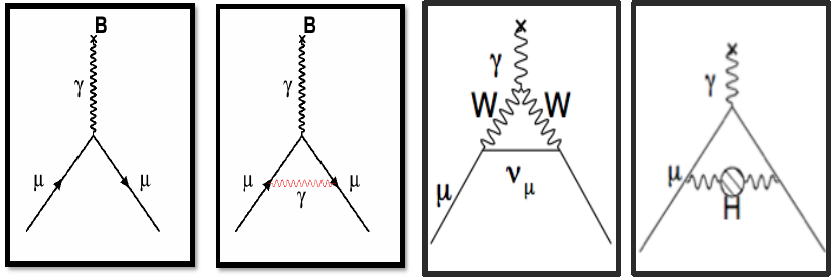
\includegraphics[width=2 cm]{a_mu_corrections.png}
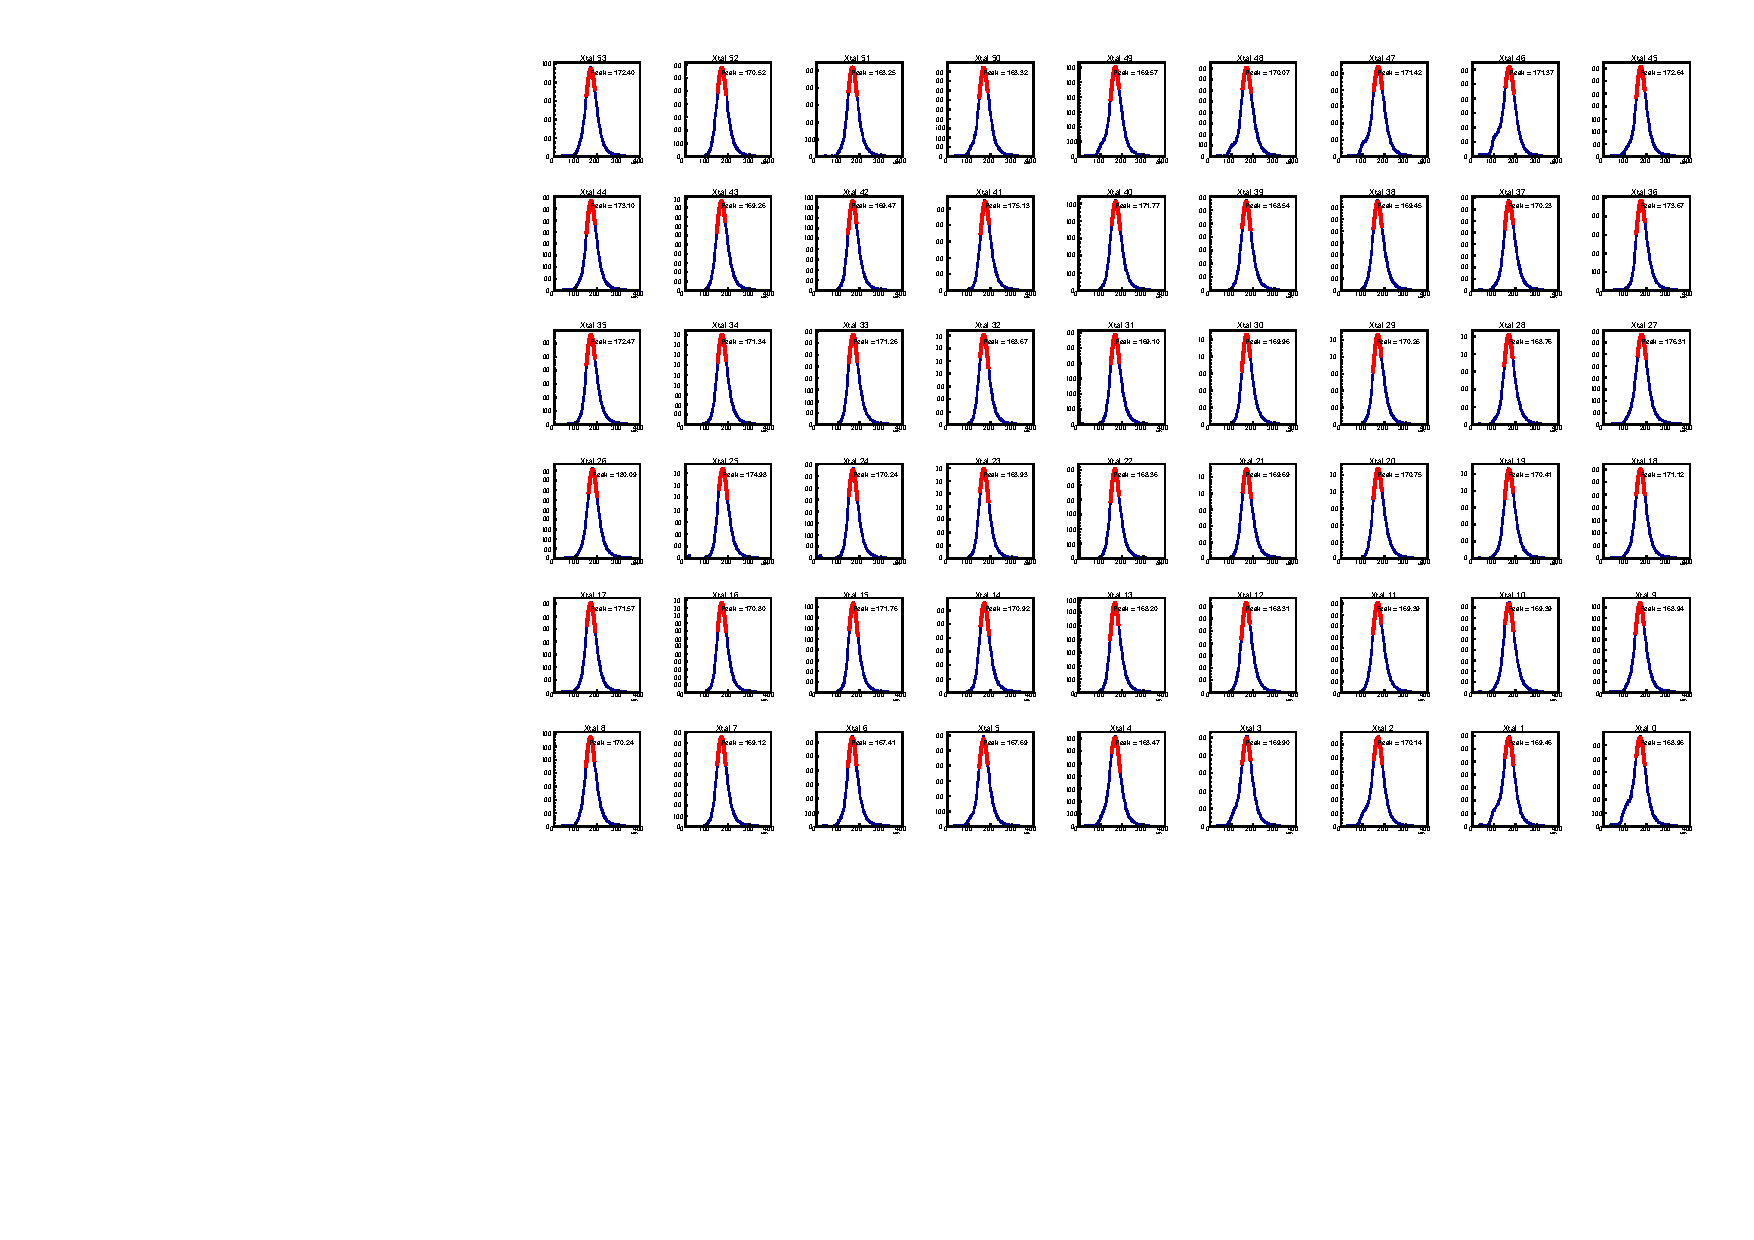
\includegraphics[width=17.2 cm]{calo1.pdf}
\caption{\label{fig4}All 54 crystals of calorimeter 1 fitted by a Gaussian about the peak to find the MIP peak. }
\end{figure} 

To understand and check the consistency of equalization, 
every crystal is fitted to a Gaussian about the peak to find the MIP peak. 
A distribution of the MIP peak of 1296 crystals is plotted for all 24 calorimeters and this is almost a Gaussian 
distribution as shown in figure \ref{fig5} for the 60--hour dataset. 
A Gaussian fit to this plot about the range as shown indicates a spread of about 
1.13\% (spread is defined as the $\sigma$/mean of the distribution). %Note the entire range is not fitted as some 
%crystals were not correctly functioning due to some hardware failure or other reasons. 
\section{Comparing the consistency of energy equalization of all crystals across various datasets}
\noindent A comparison of the MIP energy distribution of all crystals across various datasets is 
performed to check the consistency of the energy equalization. 
The datasets considered are as follows:
\begin{itemize} 
\item The 60--hour dataset.
\item The 9 days dataset which is about three times the 60--hour dataset.
\item The endgame dataset which is about three times the 9 days dataset.
\end{itemize} 

For a comparison of all calorimeters of the 60--hour dataset and 9 days dataset, two methods were used and both 
yielded similar results proving the consistency of the energy equalization and calibration of the crystals 
and functioning of the laser calibration system.
\begin{figure}[H]
\centering
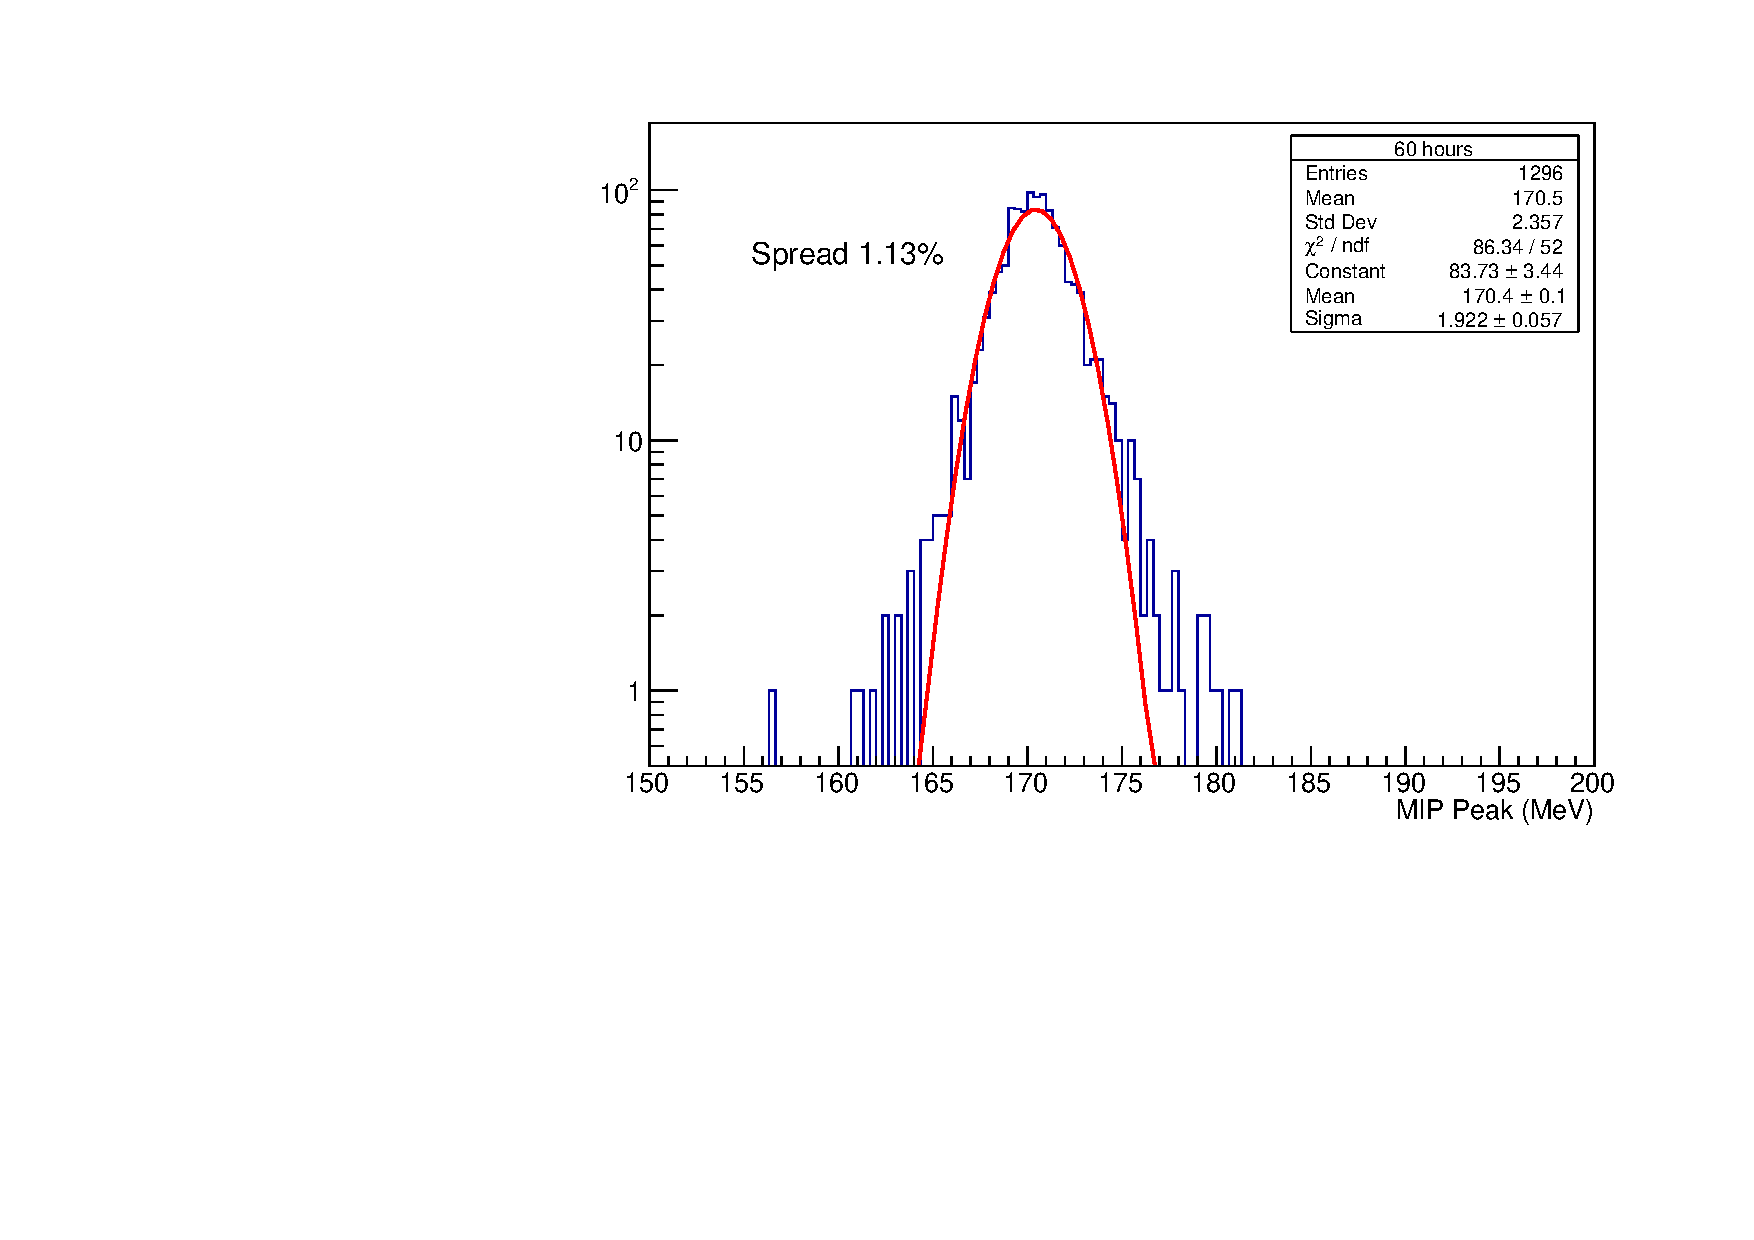
\includegraphics[width=7.2 cm]{all_xtal_1.pdf}
\caption{\label{fig5}Distribution of MIP peak of lost muons for all crystals of all calorimeters. }
\end{figure}

%The note \cite{docdb16874} explains the reason for the improper functioning of these crystals in figure \ref{fig6}.
%This holds true for all datasets of run1 as we will see in the subsequent section. 

Crystal number 22, a somewhat central crystal in the 9$\times$6 
grid structure of a calorimeter as is evident from figure \ref{fig4}, is taken to be a reference and the mean value of 
its MIP peak is plotted for each calorimeter in figure \ref{fig7} left panel. The two datasets are overlaid 
(red represents 60--hours and blue represents 9 days dataset respectively). The rms 
values in both cases (1.06 for 60--hours and 1.23 for 9 days) are similar and represented by the bands. 

\begin{figure}[H]
\centering
%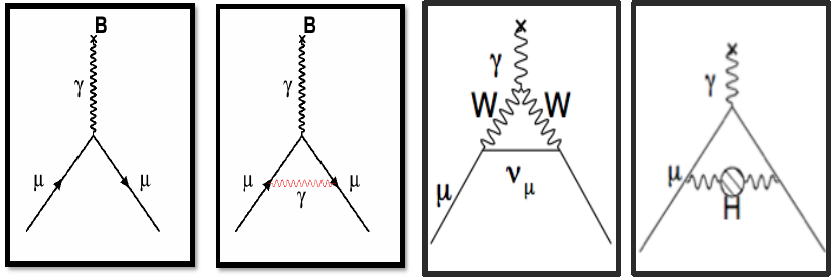
\includegraphics[width=2 cm]{a_mu_corrections.png}
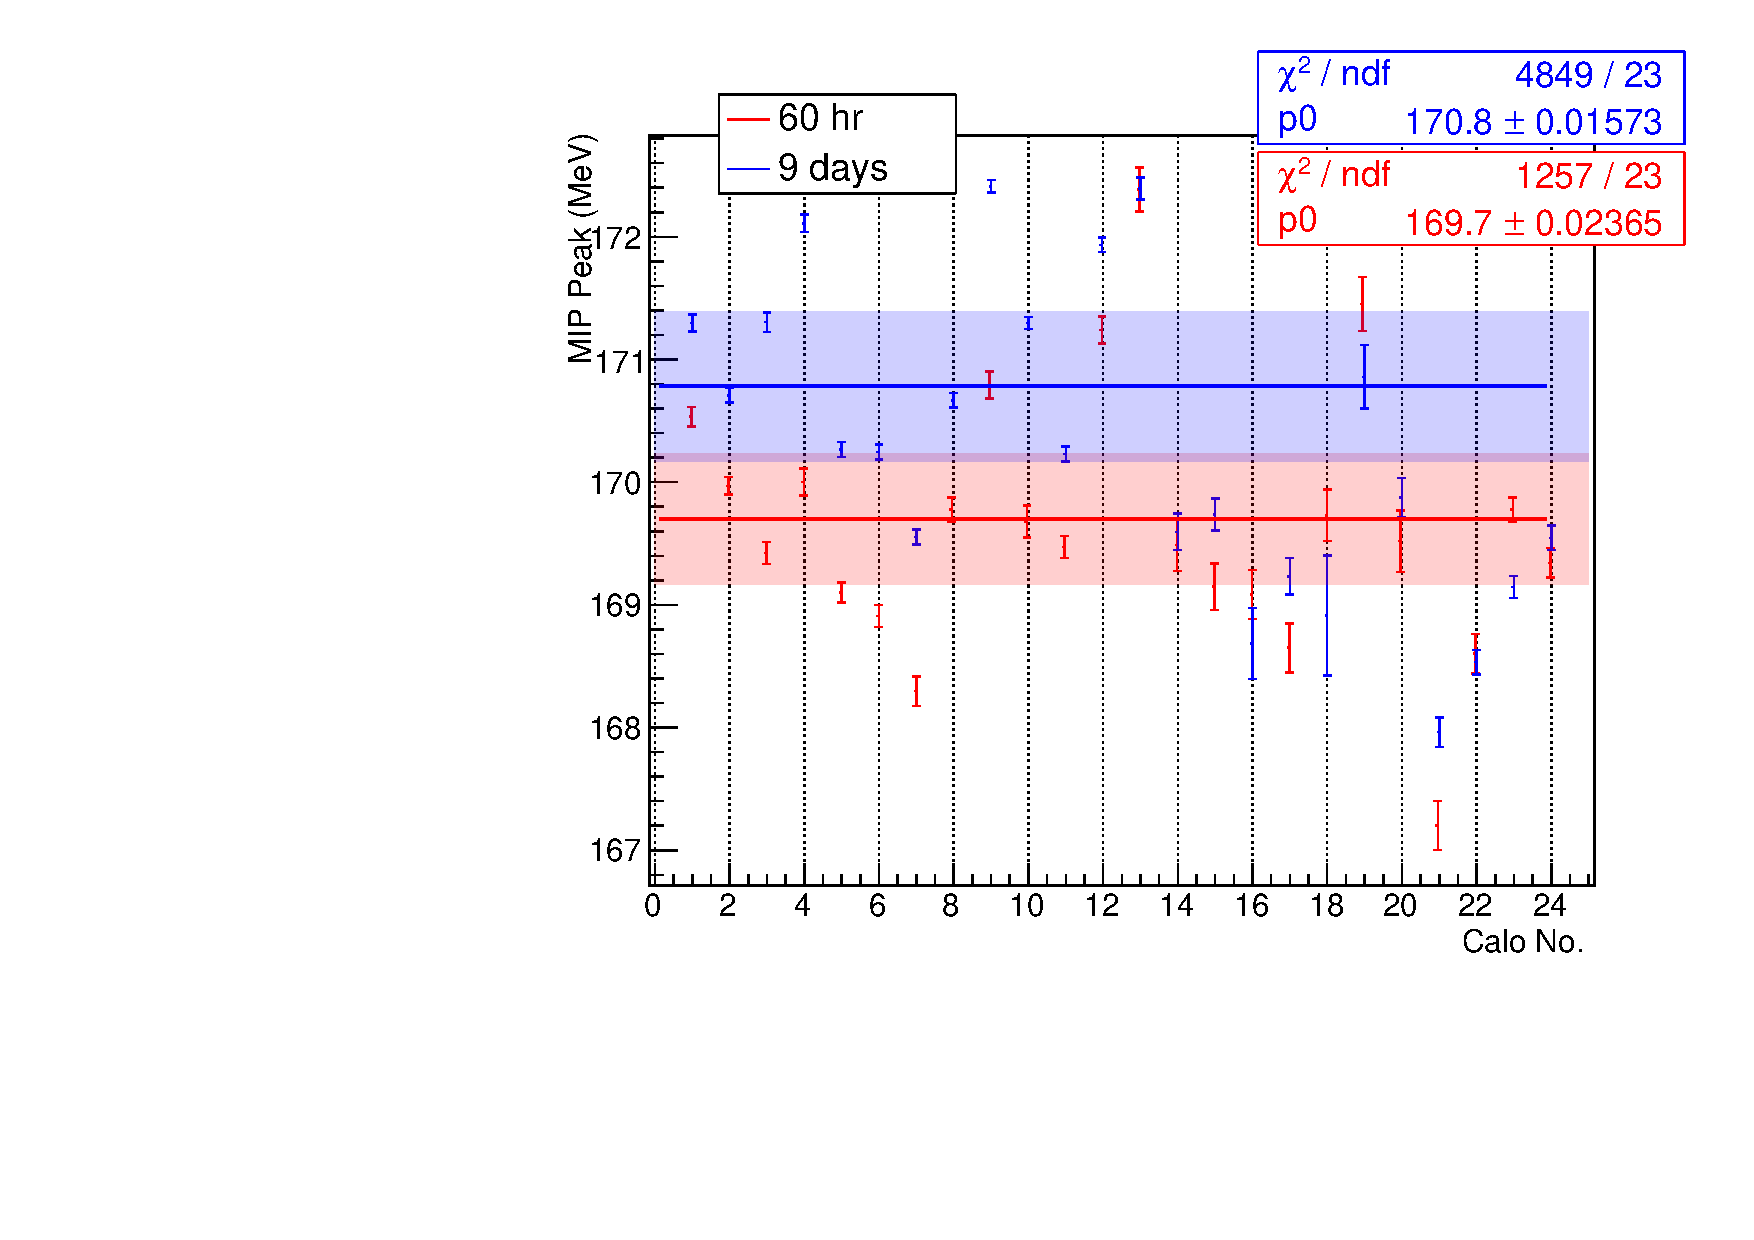
\includegraphics[width=7 cm]{allCalo_xtal22_1.pdf}
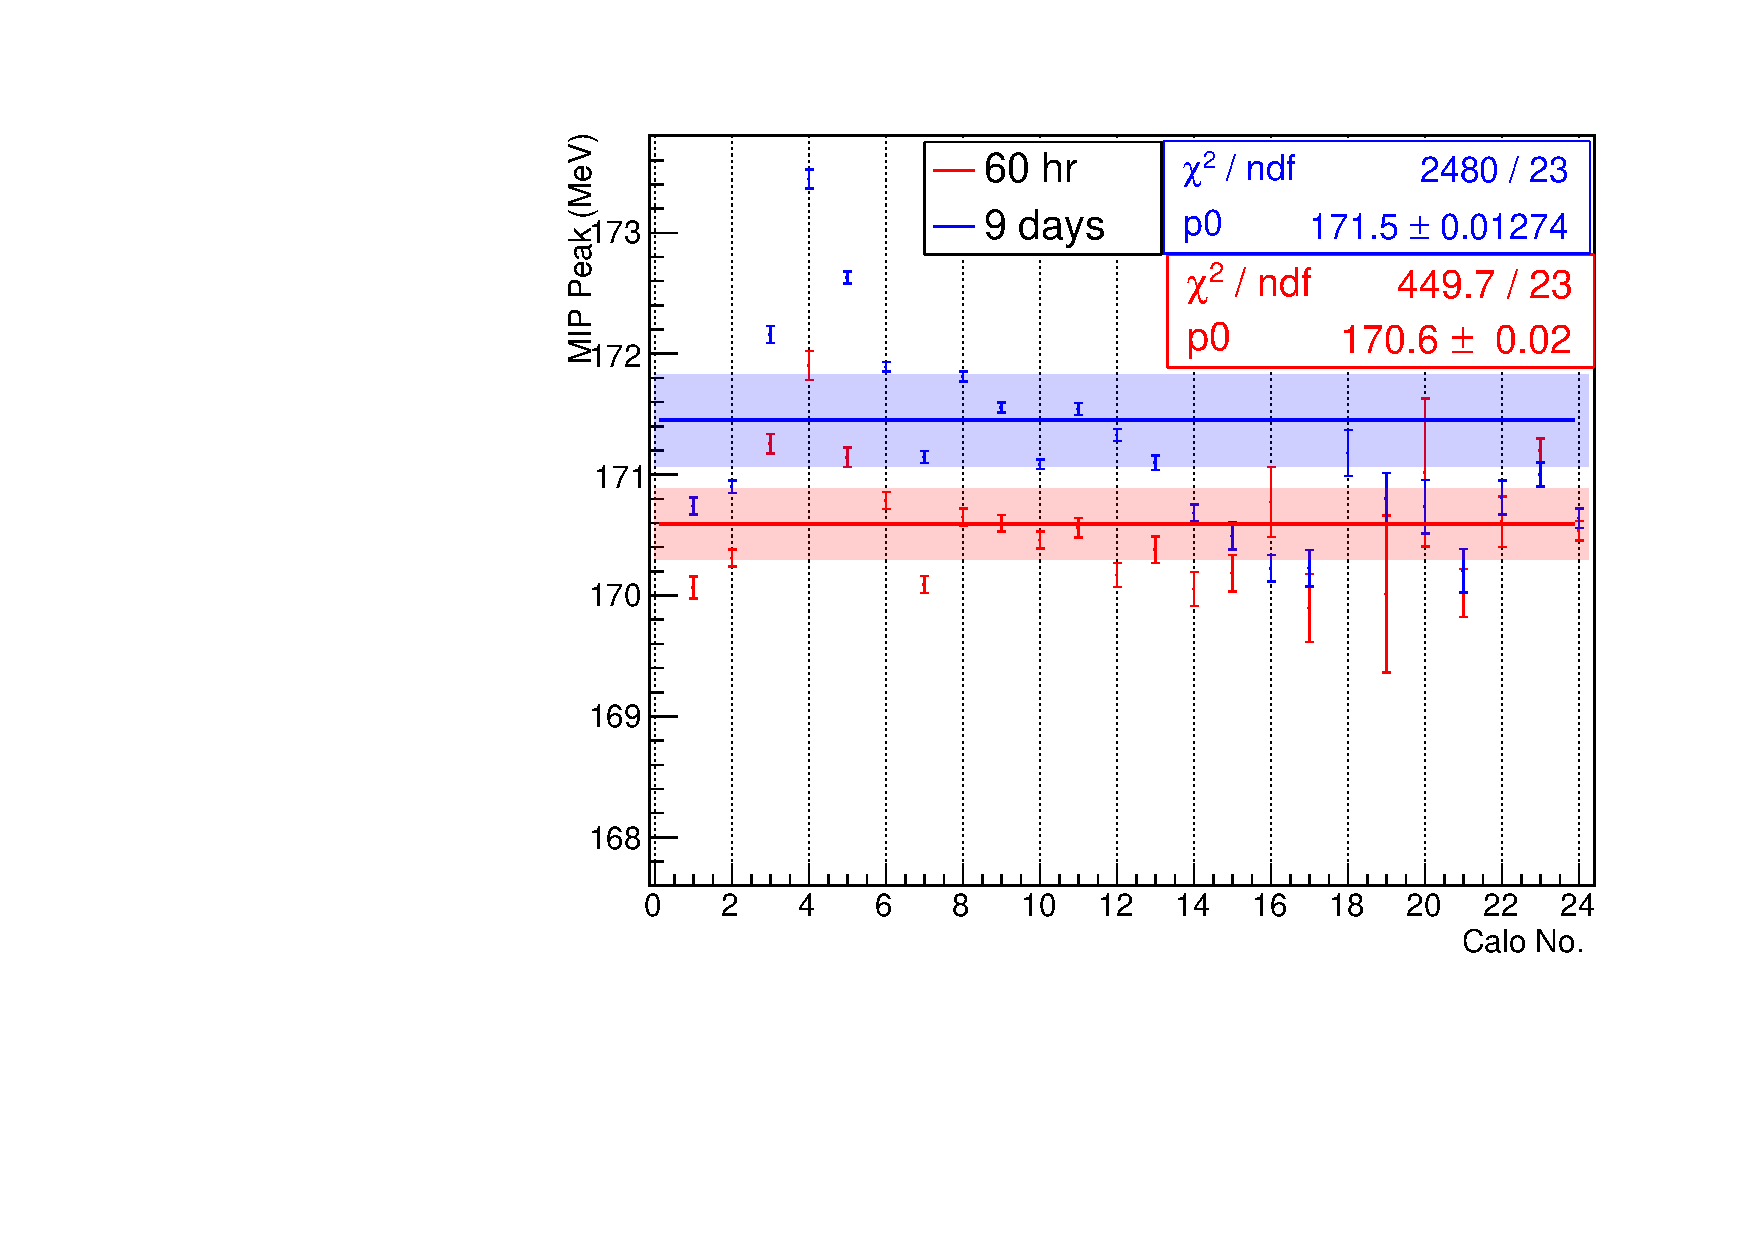
\includegraphics[width=7 cm]{allCalo_wt_1.pdf}
\caption{\label{fig7}Left: MIP peak of crystal 22 of all calorimeters for 60--hours (in red) and 9 days (in blue) dataset. 
Right: MIP peak of the average of all the crystals of each calorimeter for 60--hours 
(in red) and 9 days (in blue) dataset. }
\end{figure}  

The right panel of figure \ref{fig7} compares the average of all crystals of a calorimeter. 
It is ensured that each crystal has an equal number of lost muon event. 
This average of the MIP peak is plotted for each calorimeter. The rms 
values in both cases here are 0.6 for 60--hours and 0.76 for 9 days respectively. The mean values of the MIP 
peaks in both the left and right panels are also of similar magnitude. 

Finally, the distributions of MIP peaks of all crystals for all the three datasets are overlaid for comparison 
as shown in the left panel of figure \ref{fig8}. They show a similar trend but the spread is maximum for the endgame 
dataset (in black). This could be owing to higher statistics accumulated for a much longer period of time 
(the gains could be influenced by some environmental like temperature, humidity, etc. for longer time periods). 
The spreads of the 60--hour, 9 days and endgame datasets are 1.13\%, 1.33\% and 1.5\% respectively. 

%%%%%%%%%%%%%%%%%%%%%%%%%%%%%%%%%%%%%%%%%%
  
%%%%%%%%%%%%%%%%%%%%%%%%%%%%%%%%%%%%%%%%%%

\section{Defining new equalization constants}
\noindent The maximum spread of the MIP energy observed in run 1 data is of the order of 1.5\%. This 
is less than the 3\% fluctuation in the endpoint energy of 3.1 MeV of the positron spectrum \cite{c2}. 
Nevertheless, a further correction with new equalization constants is devised 
to check for a scope of further improvement. 
 
 
This is tested by investigating  the distribution of the ratio of MIP peaks of two different datasets. The 60--hours 
and 9 days datasets are chosen for this purpose. Thus the distribution of $MIP_{9d}:MIP_{60h}$ (which 
should be centered around unity) as shown in the middle panel of figure \ref{fig8} is plotted. 
\begin{figure}[H]
\centering
%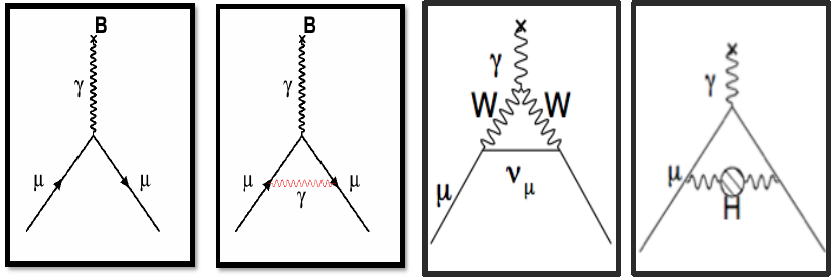
\includegraphics[width=2 cm]{a_mu_corrections.png}
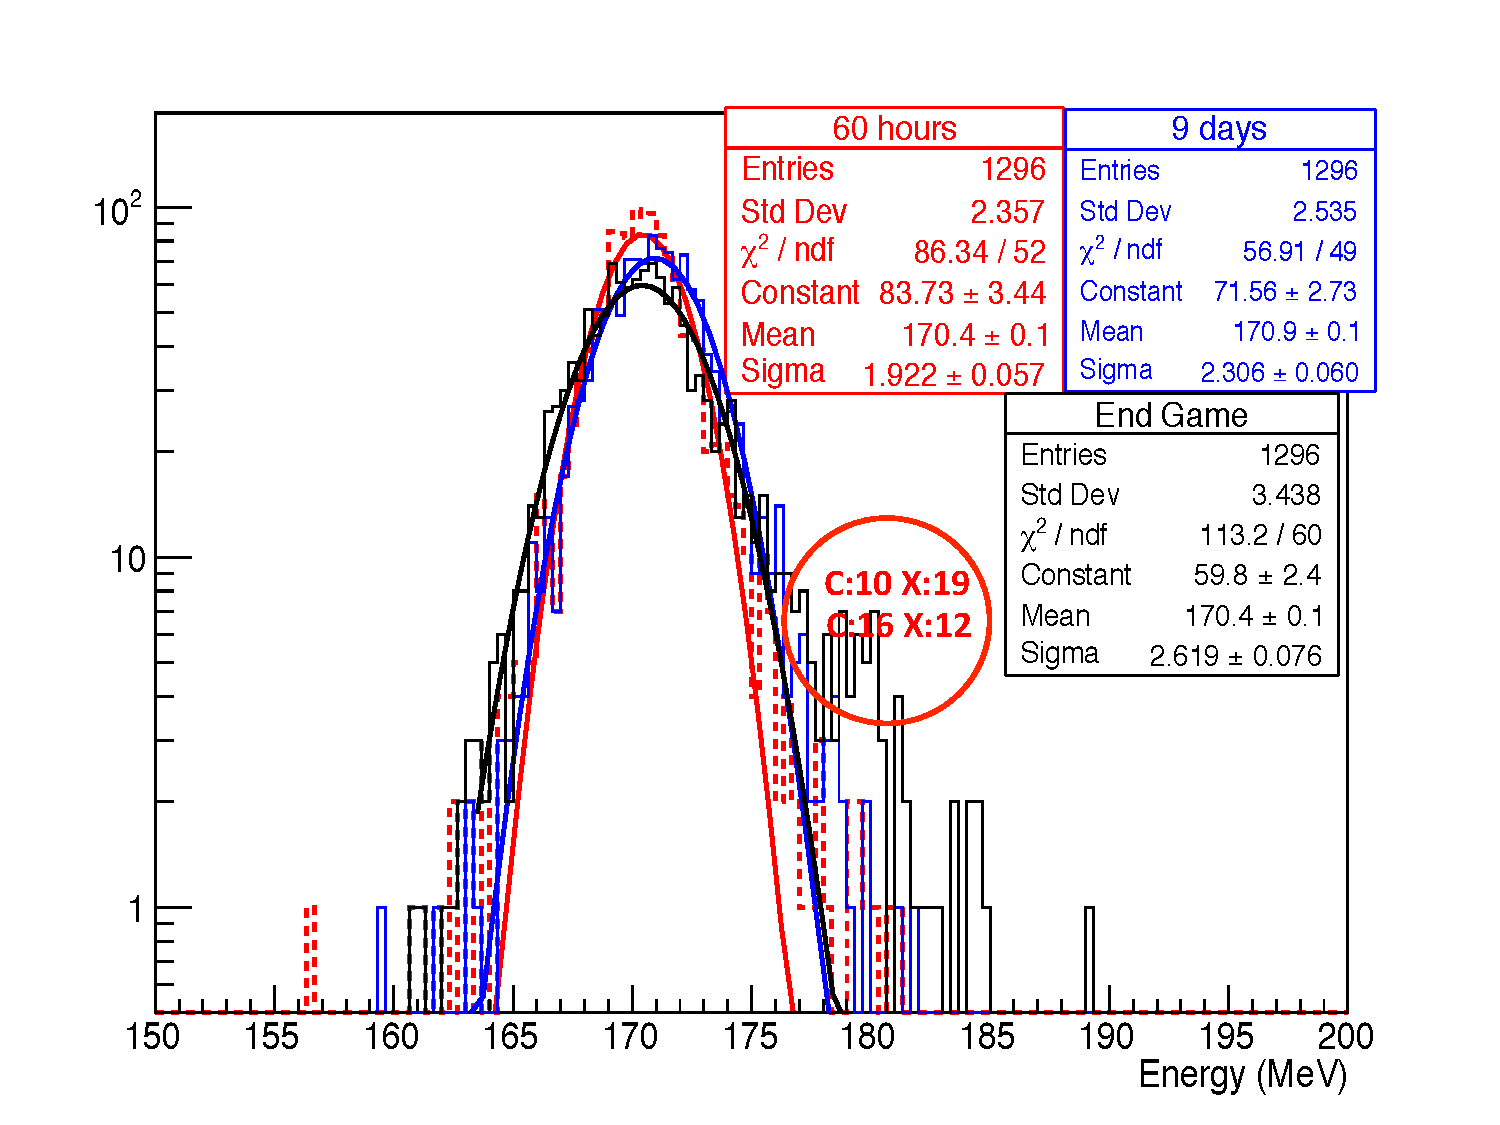
\includegraphics[width=5.3 cm]{comp_all_1.pdf}
\includegraphics[width=4.8 cm]{ratio.pdf}
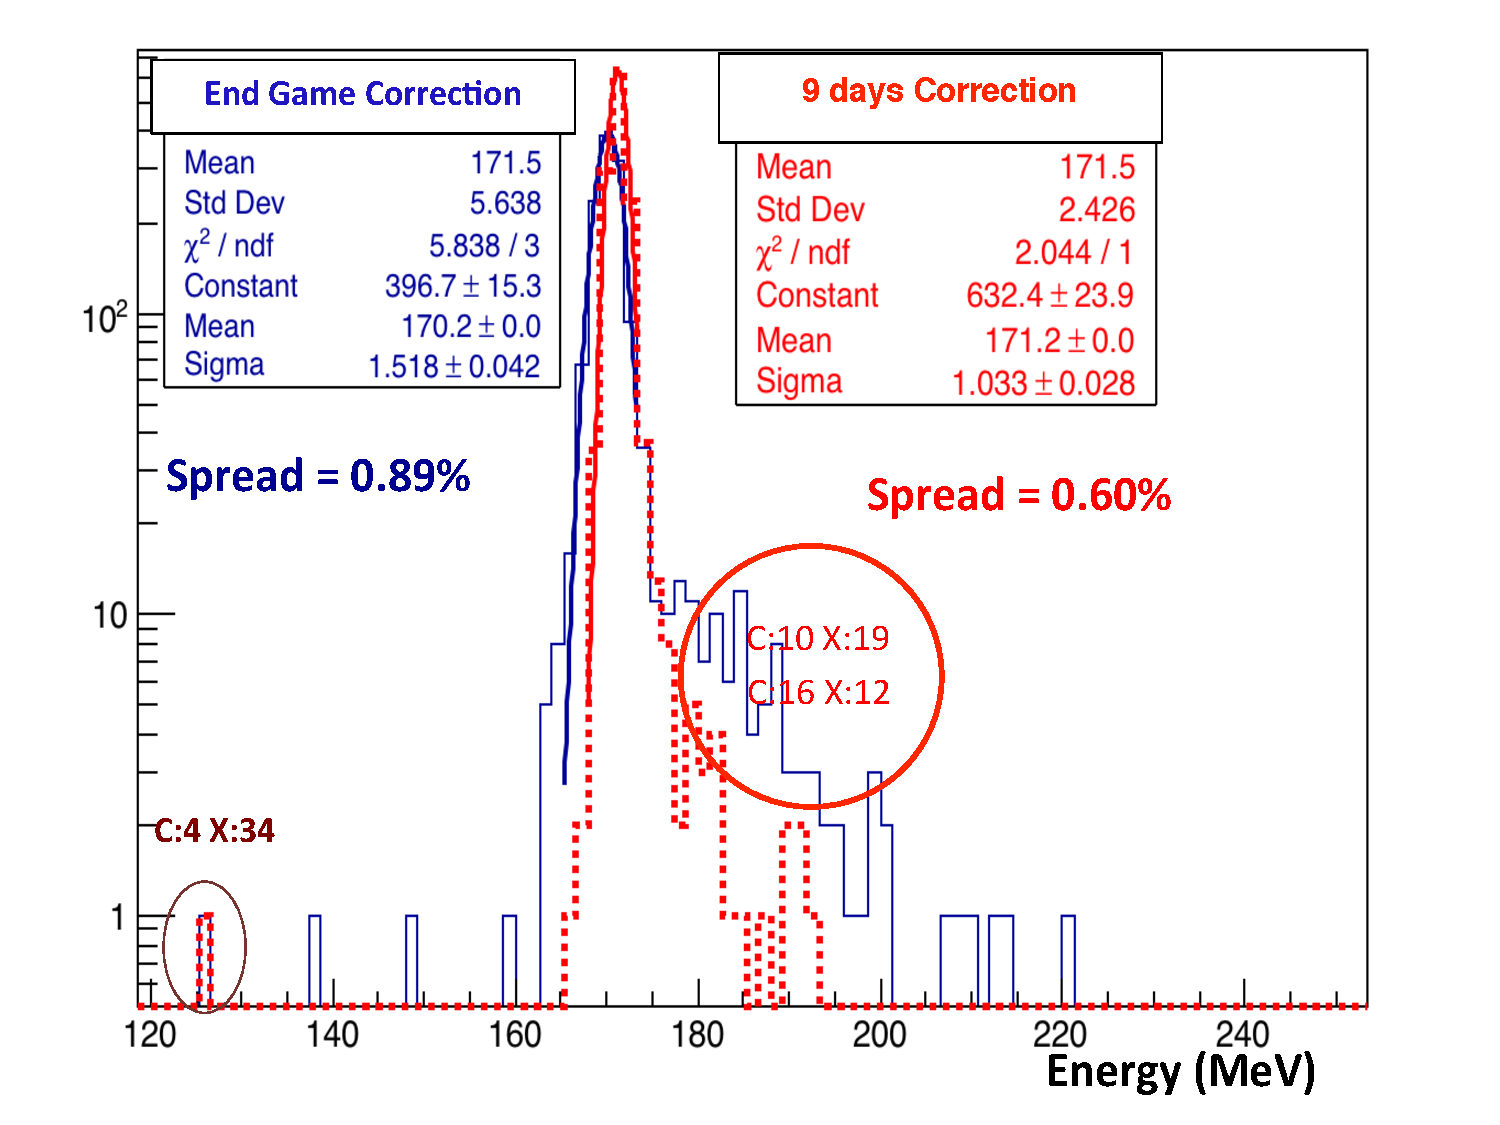
\includegraphics[width=5.1 cm]{comp_corr.pdf}
%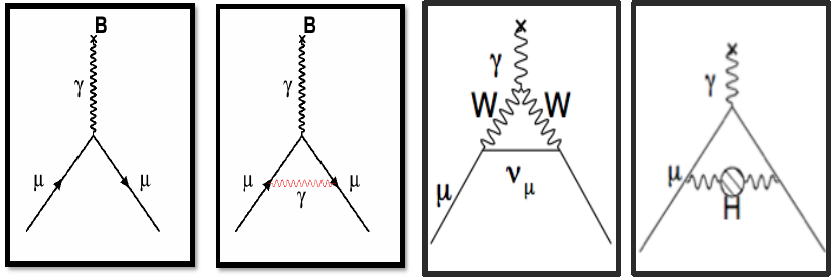
\includegraphics{a_mu_corrections.pdf}
\caption{\label{fig8}Left: MIP peak distribution of all 1296 crystals for all datasets overlaid - 60--hours (in red), 
9 days (in blue) and endgame (in black). Middle: The distribution of $MIP_{9d}:MIP_{60h}$. Right: MIP peak distribution 
datasets overlaid - 9 days (in red) and endgame (in blue) after applying a correction factor obtained from 60--hours dataset.}
\end{figure} 
The spread of the distribution of this ratio is found to be 0.99\%, which is 
lower than the spread of the individual distributions of all the datasets respectively. 
Thus, an improvement with new equalizations constants is evident. %The same is true for any pair of ratios of datasets. 

\noindent \textbf{A brief outline of the procedure used:}\\
The 60--hour dataset is used as the reference for finding the new energy equalization constants. 
An average MIP constant for the $i^{th}$ crystal ($M_i$) is defined using $ M_i = \frac {E_i}{\langle {E_i}\rangle}$, 
where $\langle {E_i}\rangle$ is the mean value of the distribution of the MIP peaks of all crystals obtained by fitting 
a small region as shown in the left panel of figure \ref{fig8} for the 60--hour dataset. 
This constant $M_i$ is divided by the MIP peak of every crystal of the 9 days dataset and the endgame dataset 
to obtain new MIP peak for each crystal. The resultant spectrum obtained for the sum of E0, E1 and E2 were 
added and fitted with a Gaussian about the peak to obtain the MIP peak of each crystal. 
The distributions of the new MIP peaks for these two datasets are plotted in the right panel of figure \ref{fig8}. There is almost a 
50\% reduction in the spread compared to spread in the original equalization constants (refer left panel of figure \ref{fig8}).  
\begin{figure}[H]
\centering
%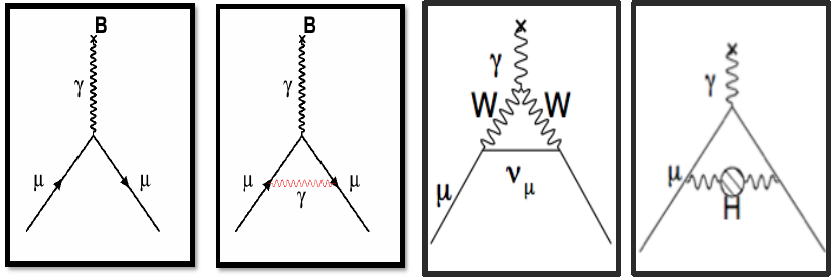
\includegraphics[width=2 cm]{a_mu_corrections.png}
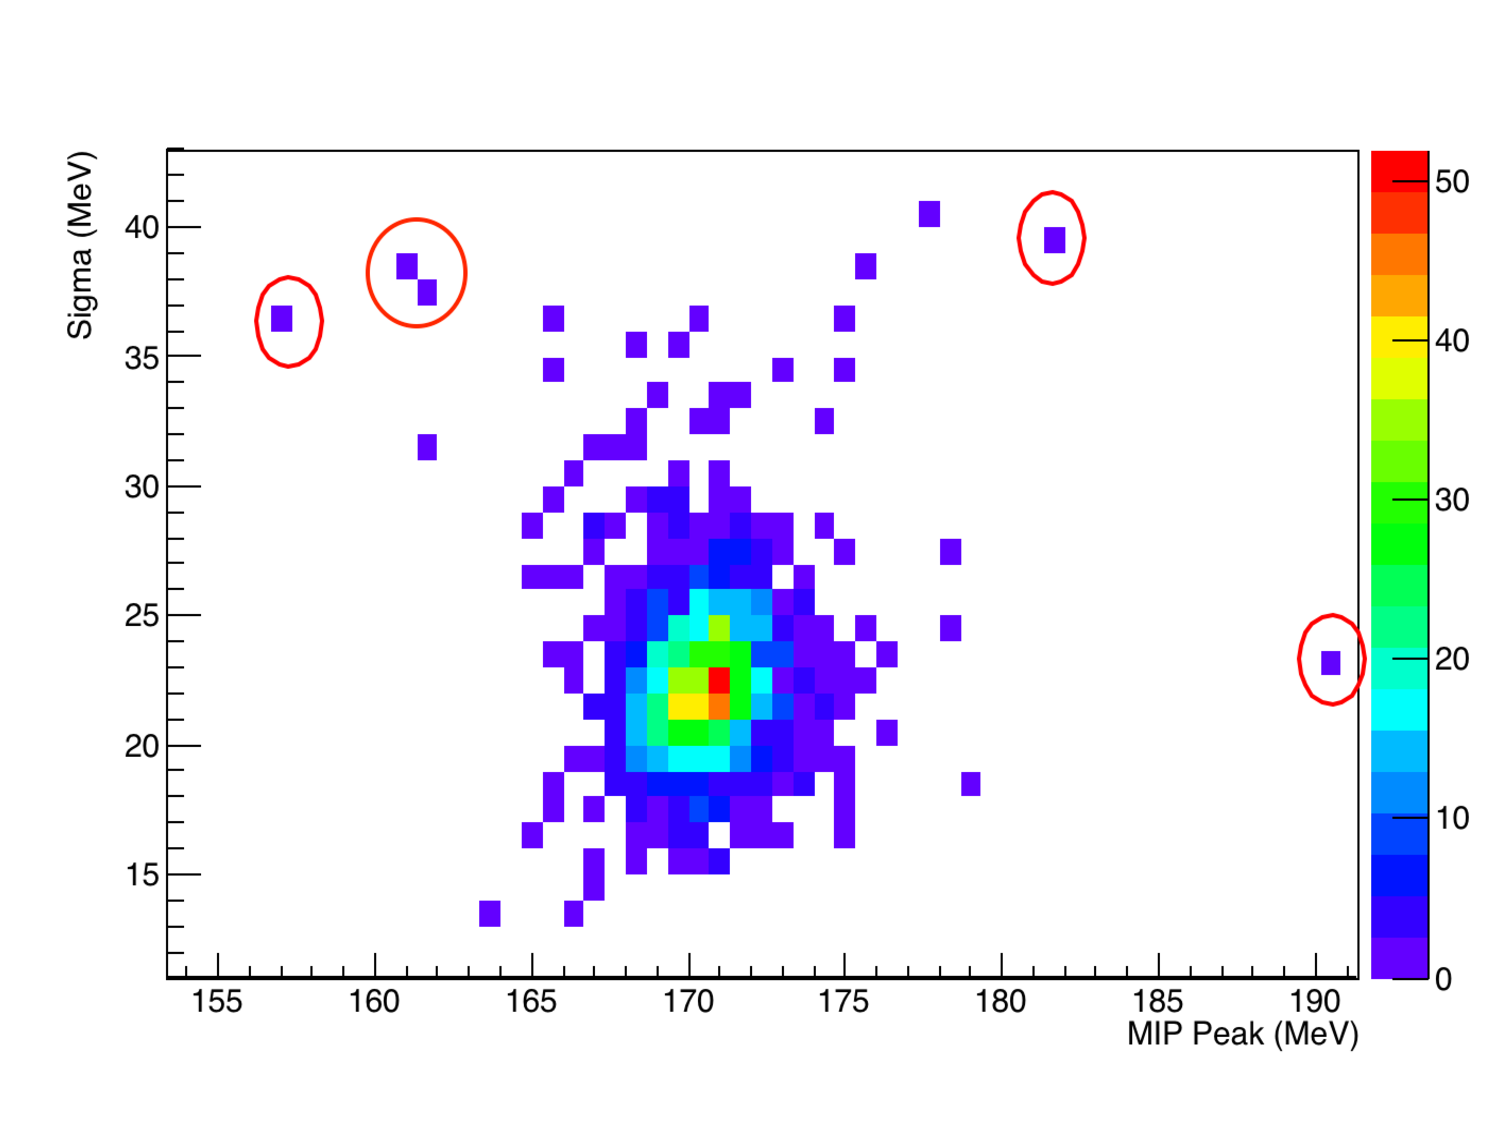
\includegraphics[width=7 cm]{sigma_mip.pdf}
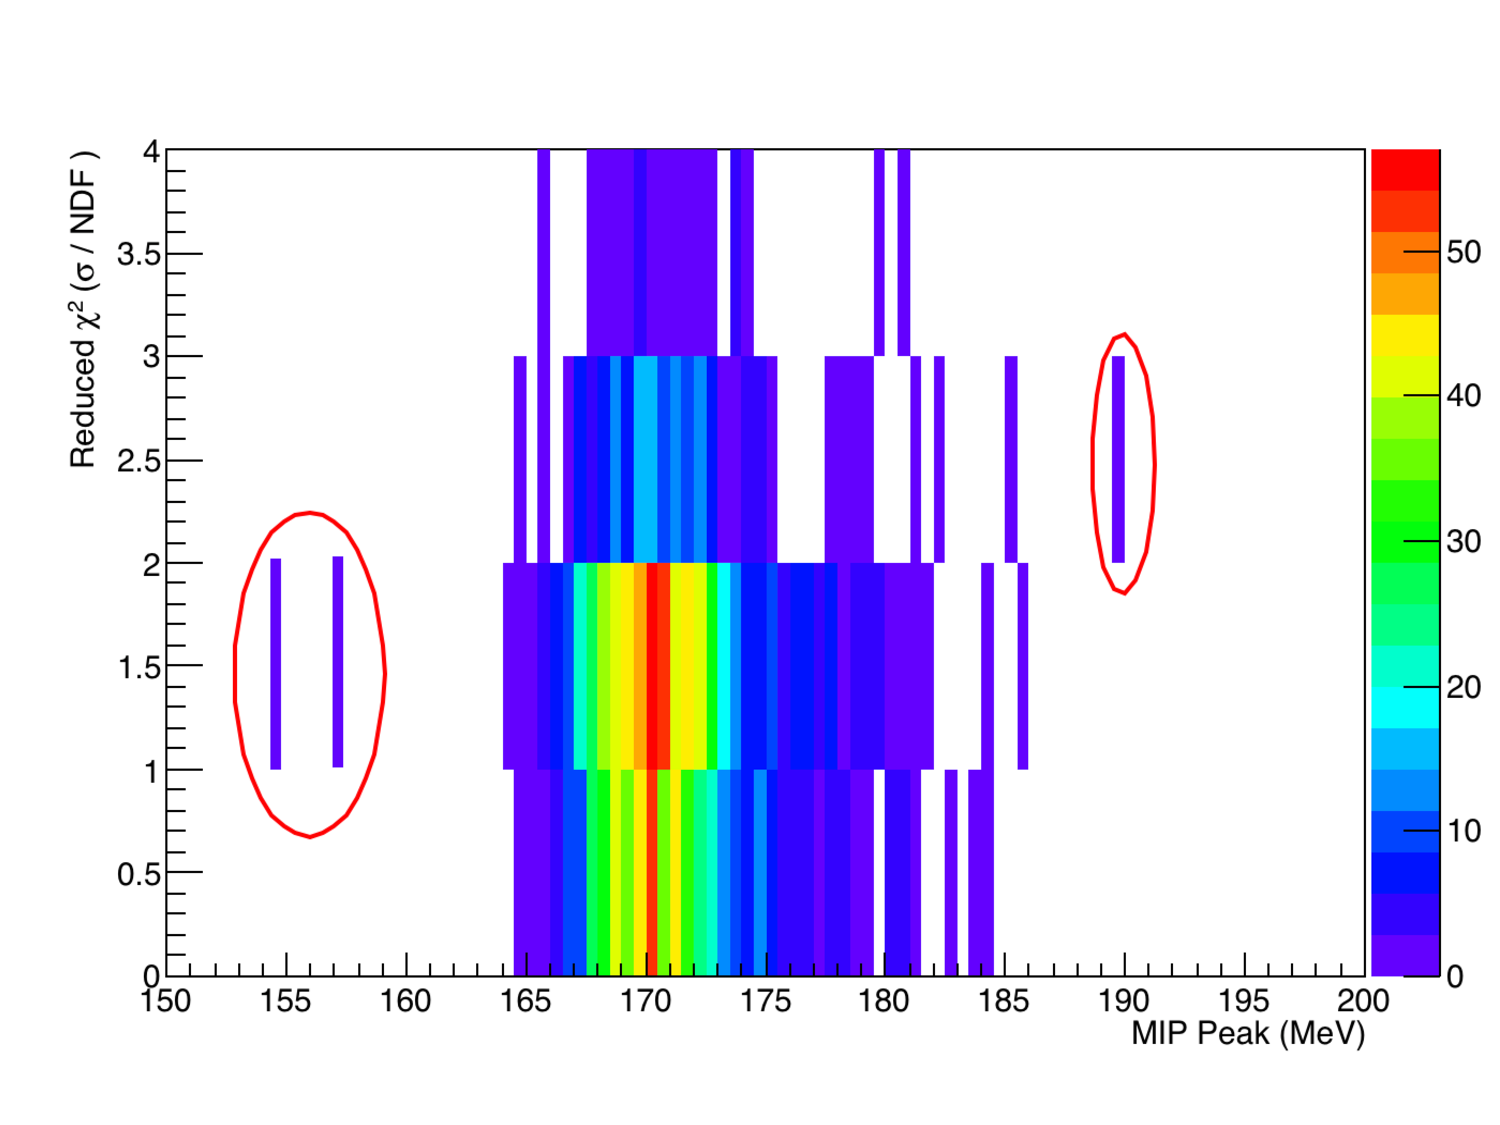
\includegraphics[width=7 cm]{chi2_mip.pdf}
\caption{\label{fig9}Left: A scatter plot of sigma versus MIP peak of the 60--hour dataset.
Right: A scatter plot of reduced $\chi^2$ versus MIP peak of the 60--hour dataset. The red circles indicate the outlier in both cases.}
\end{figure}  
The outliers or the tail region of the left and right panels of figure \ref{fig8} corresponding to a few crystals 
that have MIP peaks of lower or higher energy ranges than usual (> 180 MeV and <150 MeV). These have a 
comparatively large sigma of the Gaussian distribution as is evident in the left 
panel of the scatter plot of sigma versus MIP peak in figure \ref{fig9}. 
The reduced $\chi^2$ of these fits are also > 1 as seen in the right panel of this figure.  
A few such crystals causing the tail of the distribution shown in red circles in figure \ref{fig8} and figure \ref{fig9} 
are individually plotted in the left panel figure \ref{fig6}. 
\begin{figure}[H]%[H] places fig. in exact position
\centering
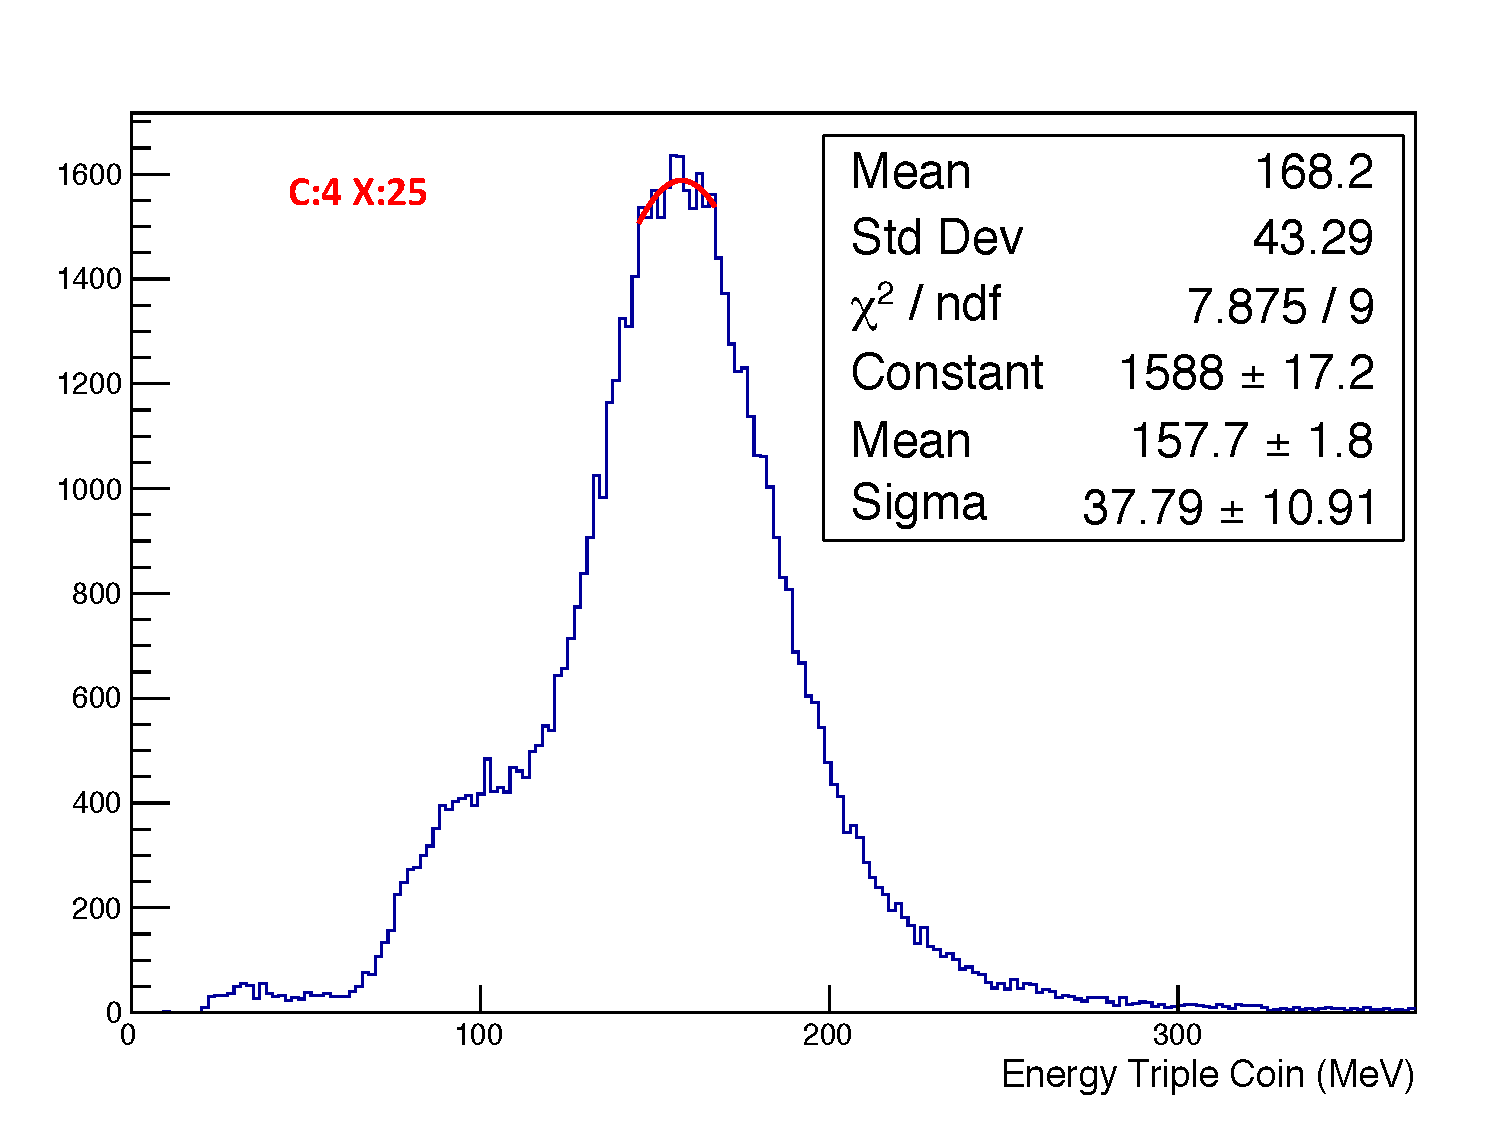
\includegraphics[width=7 cm]{c4_x25.pdf}%before
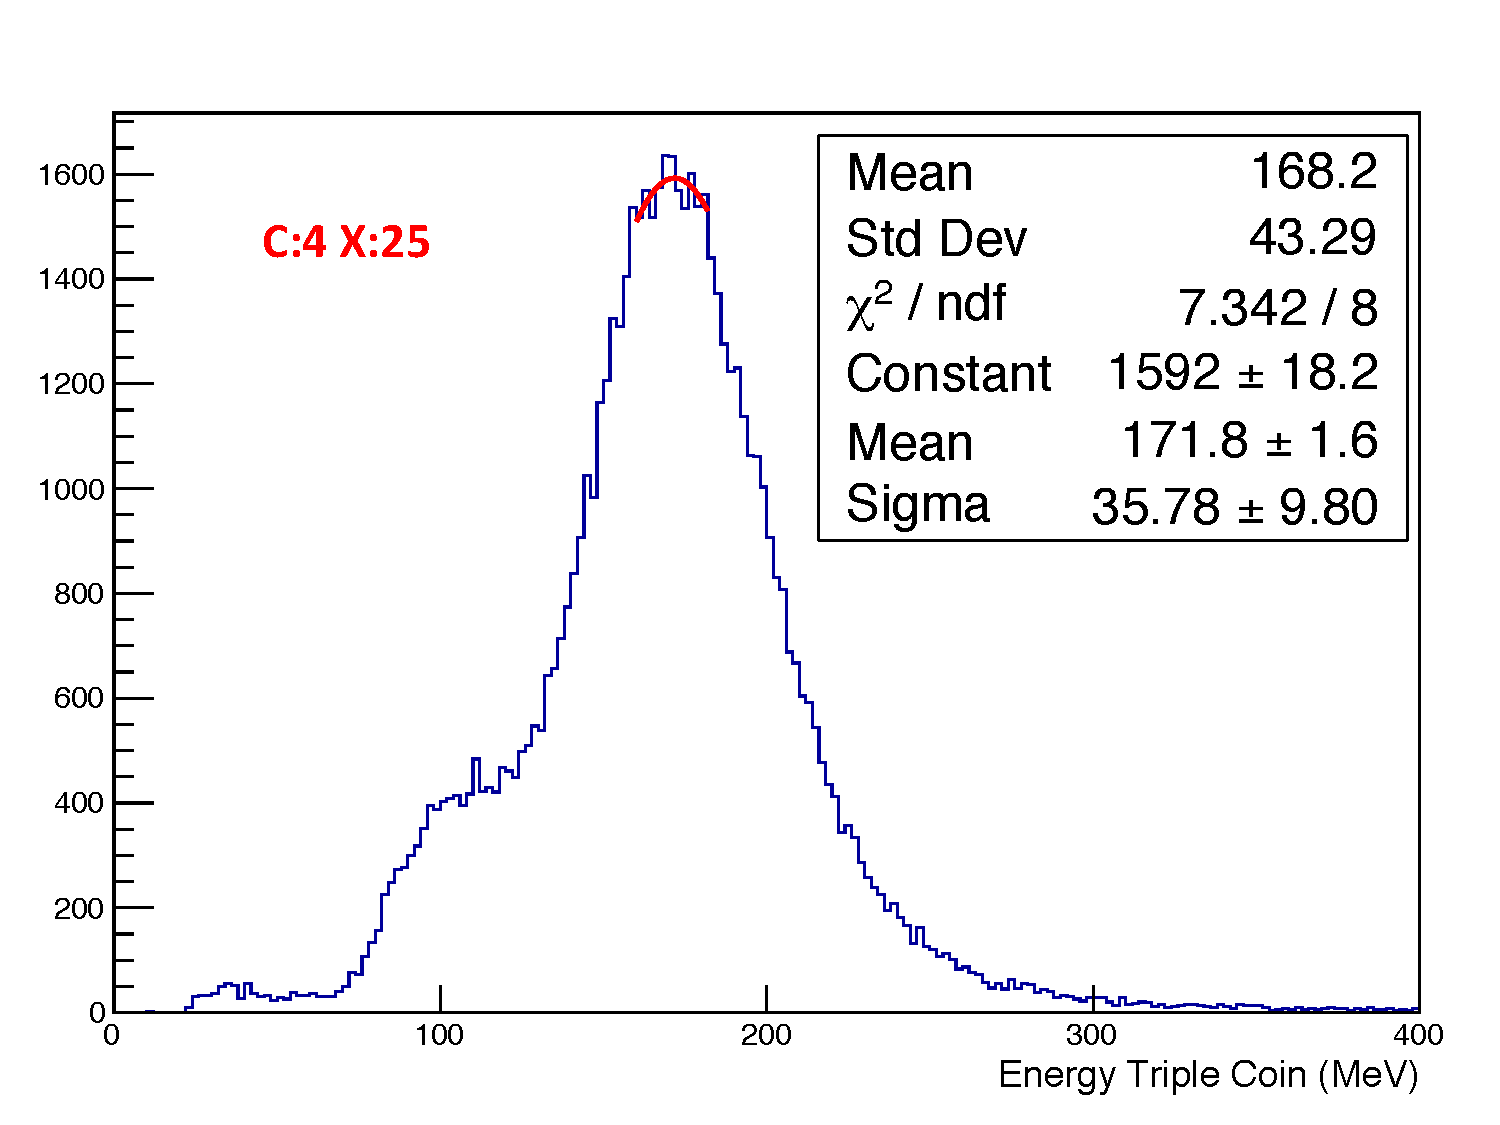
\includegraphics[width=7 cm]{c4_x25_after.pdf}\\%after
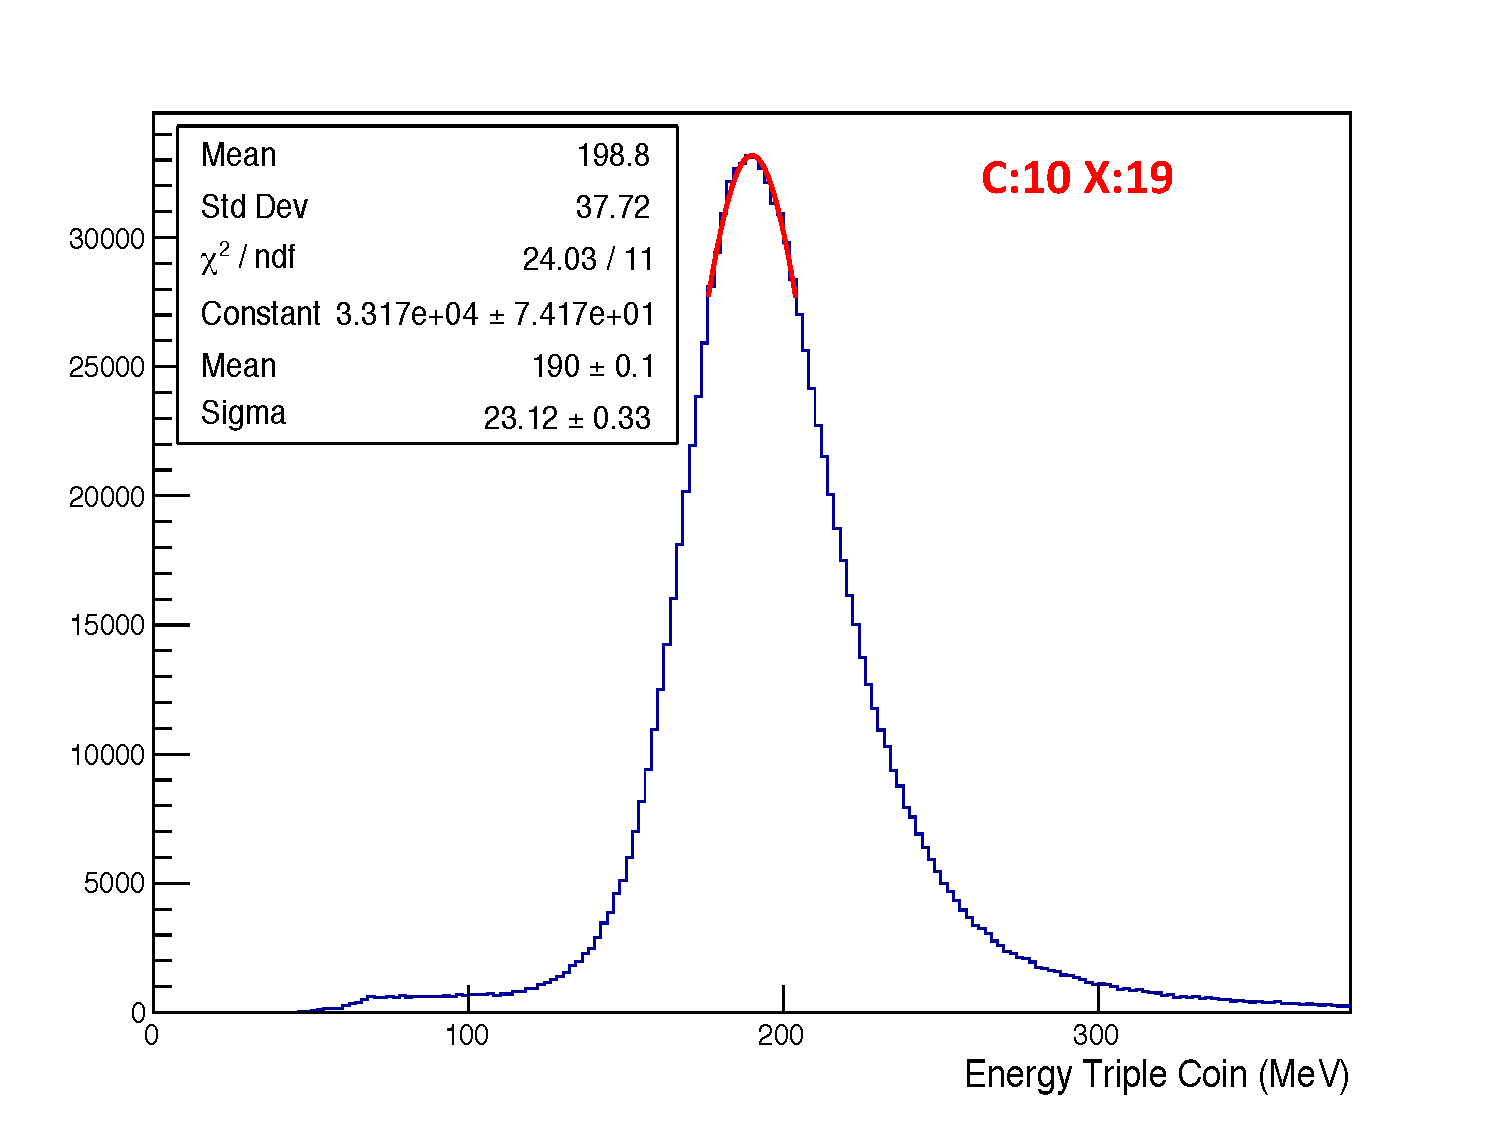
\includegraphics[width=7 cm]{c10_x19.pdf}%before
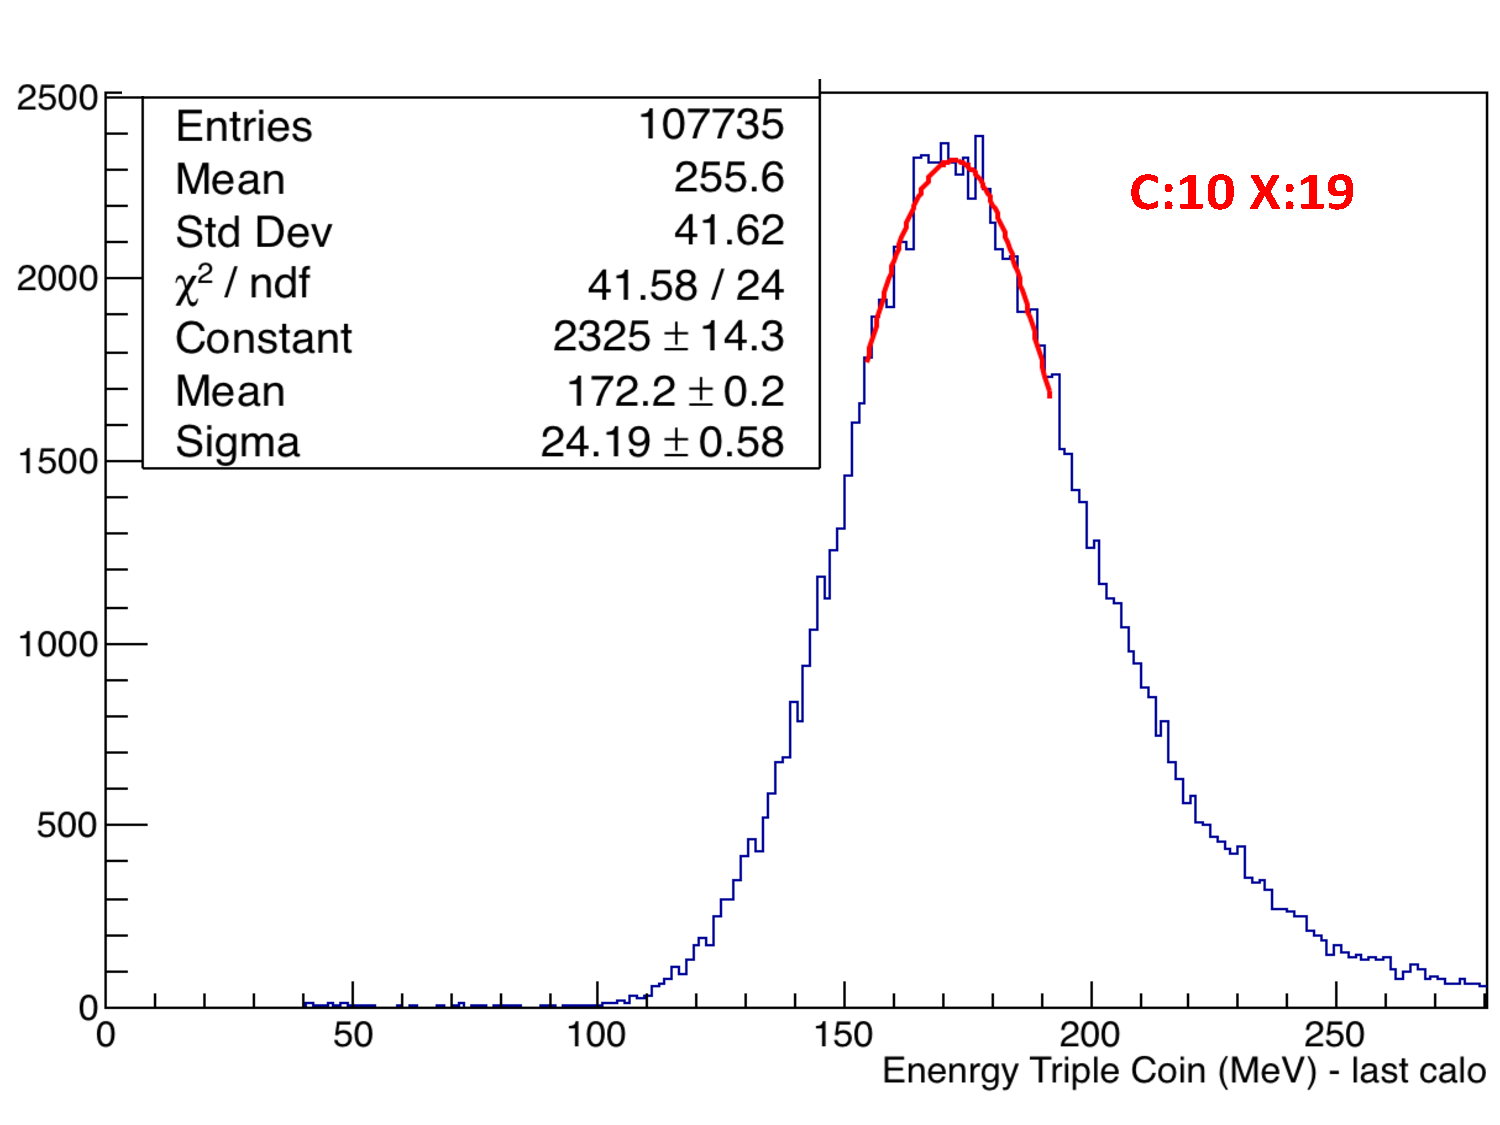
\includegraphics[width=7 cm]{c10_x19_after.pdf}\\%after
\includegraphics[width=7 cm]{c16_x12.pdf}%before
\includegraphics[width=7 cm]{c16_x12_after.pdf}\\%after
\includegraphics[width=7 cm]{c4_x34.pdf}%before
\includegraphics[width=7 cm]{c4_x34_after.pdf}%after
\caption{\label{fig6}Left: Four bad crystals showing MIP distribution before a correction. 
Right: The same crystals showing MIP distribution after an applied correction.}
\end{figure} 
\noindent These four crystals are also reported to not function properly in \cite{docdb16874}. 
Calorimeter 4 crystal 25 and crystal 34 both have a lower energy scale due to some malfunctioning -- 
for details refer \cite{docdb16874}. This proves the reliability and consistency of this study. 
The effect of the new equalization constants is especially suitable for these bad crystals. 
The right panel of figure \ref{fig6} shows the new spectrum of the triplets fitted about the peak for 
the same crystals i.e. crystal 25 of calorimeter 4, crystal 19 of calorimeter 10, crystal 12 of calorimeter 16 
and crystal 34 of calorimeter 4 respectively. Note that though the shape of the 
spectrum is the same in all cases but the MIP peak has shifted in the right direction after applying this 
second-order correction, except for crystal 34 of calorimeter 4. This is expected as this particular crystal 
is not functioning properly \cite{docdb16874}.%\textbf{Must find the prob. in docdb 16874 probably}
\section{Conclusions}
\noindent The final conclusions of these studies were as follows:
\begin{itemize}
\item The MIP energy distribution is quite stable for all crystals for these datasets i.e. 60--hours, 9 days and endgame and shows 
a maximum spread of 1.5\%. This is less than the 3\% fluctuation in the endpoint energy of 3.1 MeV – which
 means that the lost muons are suitable for energy equalization and calibration\cite{c2}. 
\item Detected misbehaving crystals with an anomalous MIP peak which are calorimeter 4 crystal 25, calorimeter 4 crystal 34, 
calorimeter 10 crystal 19 and calorimeter 16 crystal 12 for all 
datasets studied – this matches the studies of \cite{docdb16874}. 
\item A tail in the Gaussian distribution of the MIP peaks increases the sigma of the distribution, resulting in a slightly bad fit 
and a relatively higher reduced $\chi^2$ -- these correspond to the badly behaving crystals. 
\item A distribution of the ratio of $MIP_{9d}:MIP_{60h}$ has a spread <1\% which proves that an additional correction will 
improve the MIP distribution. 
\item Applied an additional equalization that improves MIP distribution or equalization 
in general by almost 50\% for 9 days and endgame dataset ( using  the 60--hour dataset to find the new constants).
%\item The statble results prove the correct and stable working of the laser calibration system.
\end{itemize} 

\section*{Acknowledgments}
\noindent I would like to express my gratitude to Anna Driutti who helped me with the production of these datasets. 
Besides, I also appreciate the valuable suggestions given by Stefano di Falco, Graziano Venanzoni, Franco Bedeschi 
and several others of our Italian g-2 group. 

%%%%%%%%%%%%%%%%%%%%%%%%%%%%%%%%%%%%%%%%%%
%=====================================
% References, variant A: internal bibliography
%=====================================
\reftitle{References}
\begin{thebibliography}{999}
% Reference 1
\bibitem{TDR}
J. Grange, et al. Fermilab. Muon (g-2) Technical Design Report: -FN0992-E.
\bibitem{c3}
M. Tanabashi et al. {\em Particle Data Group. Phys. Rev., D:98:030001, 2018.}
\bibitem{docdb16402}
M. Sorbara et al. {\em E989 Note 168: Lost Muon correction for $\omega_a$-europa analysis.}
\bibitem{docdb16874}
Kim Siang Khaw {\em Docdb 16874: Positron/muon based STDP study.}
\bibitem{c2}
C. Polly, BNL {\em Muon g-2 Note No. 420.} {2005}
% Reference 2
%\bibitem[Author2(year)]{ref-book}
%Author2, L. The title of the cited contribution. In {\em The Book Title}; Editor1, F., Editor2, A., Eds.; 
%Publishing House: City, Country, 2007; pp. 32-58, ISBN.
\end{thebibliography}

\end{document}
